\documentclass[a4paper]{article}
% Этот шаблон документа разработан в 2014 году
% Данилом Фёдоровых (danil@fedorovykh.ru) 
% для использования в курсе 
% <<Документы и презентации в \LaTeX>>, записанном НИУ ВШЭ
% для Coursera.org: http://coursera.org/course/latex .
% Исходная версия шаблона --- 
% https://www.writelatex.com/coursera/latex/5.3

% В этом документе преамбула

\usepackage{siunitx}
%%% Работа с русским языком
%\usepackage{cmap}					% поиск в PDF
%\usepackage{mathtext} 				% русские буквы в формулах
%\usepackage[T2A]{fontenc}			% кодировка
%\usepackage[utf8]{inputenc}			% кодировка исходного текста
%\usepackage[english,russian]{babel}	% локализация и переносы
%\usepackage{indentfirst}
%\frenchspacing
%
%\renewcommand{\epsilon}{\ensuremath{\varepsilon}}
%\newcommand{\phibackup}{\ensuremath{\phi}}
%\renewcommand{\phi}{\ensuremath{\varphi}}
%\renewcommand{\varphi}{\ensuremath{\phibackup}}
%\renewcommand{\kappa}{\ensuremath{\varkappa}}
%\renewcommand{\le}{\ensuremath{\leqslant}}
%\renewcommand{\leq}{\ensuremath{\leqslant}}
%\renewcommand{\ge}{\ensuremath{\geqslant}}
%\renewcommand{\geq}{\ensuremath{\geqslant}}
%\renewcommand{\emptyset}{\varnothing}
%\renewcommand{\Im}{\operatorname{Im}}
%\renewcommand{\Re}{\operatorname{Re}}


%%% Дополнительная работа с математикой
\usepackage{amsmath,amsfonts,amssymb,amsthm,mathtools} % AMS
%\usepackage{icomma} % "Умная" запятая: $0,2$ --- число, $0, 2$ --- перечисление

%% Номера формул
%\mathtoolsset{showonlyrefs=true} % Показывать номера только у тех формул, на которые есть \eqref{} в тексте.
%\usepackage{leqno} % Нумереация формул слева

%% Свои команды
\DeclareMathOperator{\sgn}{\mathop{sgn}}
\DeclareMathOperator{\sign}{\mathop{sign}}
\DeclareMathOperator*{\res}{\mathop{res}}
\DeclareMathOperator*{\tr}{\mathop{tr}}
\DeclareMathOperator*{\rot}{\mathop{rot}}
\DeclareMathOperator*{\divop}{\mathop{div}}
\DeclareMathOperator*{\grad}{\mathop{grad}}

%% Перенос знаков в формулах (по Львовскому)
\newcommand*{\hm}[1]{#1\nobreak\discretionary{}
{\hbox{$\mathsurround=0pt #1$}}{}}

%%% Работа с картинками
\usepackage{graphicx}  % Для вставки рисунков
\graphicspath{{figures/}}  % папки с картинками
\setlength\fboxsep{3pt} % Отступ рамки \fbox{} от рисунка
\setlength\fboxrule{1pt} % Толщина линий рамки \fbox{}
\usepackage{wrapfig} % Обтекание рисунков текстом

%%% Работа с таблицами
\usepackage{array,tabularx,tabulary,booktabs} % Дополнительная работа с таблицами
\usepackage{longtable}  % Длинные таблицы
\usepackage{multirow} % Слияние строк в таблице

%%% Теоремы
\theoremstyle{plain} % Это стиль по умолчанию, его можно не переопределять.
\newtheorem{thm}{Теорема}
\newtheorem*{thm*}{Теорема}
\newtheorem{prop}{Предложение}
\newtheorem*{prop*}{Предложение}
 
\theoremstyle{definition} % "Определение"
%\newtheorem{corollary}{Следствие}[theorem]
\newtheorem{dfn}{Определение}
\newtheorem*{dfn*}{Определение}
\newtheorem{prob}{Задача}
\newtheorem*{prob*}{Задача}

 
\theoremstyle{remark} % "Примечание"
\newtheorem*{sol}{Решение}
\newtheorem*{rem}{Замечание}

%%% Программирование
\usepackage{etoolbox} % логические операторы

%%% Страница
%\usepackage{extsizes} % Возможность сделать 14-й шрифт
%\usepackage{geometry} % Простой способ задавать поля
%	\geometry{top=25mm}
%	\geometry{bottom=35mm}
%	\geometry{left=35mm}
%	\geometry{right=20mm}
 
\usepackage{fancyhdr} % Колонтитулы
%	\pagestyle{fancy}
 %	\renewcommand{\headrulewidth}{0pt}  % Толщина линейки, отчеркивающей верхний колонтитул
	%\lfoot{Нижний левый}
	%\rfoot{Нижний правый}
	%\rhead{Верхний правый}
	%\chead{Верхний в центре}
	%\lhead{Верхний левый}
	%\cfoot{Нижний в центре} % По умолчанию здесь номер страницы

\usepackage{setspace} % Интерлиньяж
%\onehalfspacing % Интерлиньяж 1.5
%\doublespacing % Интерлиньяж 2
%\singlespacing % Интерлиньяж 1

\usepackage{lastpage} % Узнать, сколько всего страниц в документе.

\usepackage{soul} % Модификаторы начертания

\usepackage{hyperref}
\usepackage[usenames,dvipsnames,svgnames,table,rgb]{xcolor}
\hypersetup{				% Гиперссылки
    unicode=true,           % русские буквы в раздела PDF
    pdftitle={Заголовок},   % Заголовок
    pdfauthor={Автор},      % Автор
    pdfsubject={Тема},      % Тема
    pdfcreator={Создатель}, % Создатель
    pdfproducer={Производитель}, % Производитель
    pdfkeywords={keyword1} {key2} {key3}, % Ключевые слова
%    colorlinks=true,       	% false: ссылки в рамках; true: цветные ссылки
    %linkcolor=red,          % внутренние ссылки
    %citecolor=black,        % на библиографию
    %filecolor=magenta,      % на файлы
    %urlcolor=cyan           % на URL
}

\usepackage{csquotes} % Еще инструменты для ссылок

%\usepackage[style=apa,maxcitenames=2,backend=biber,sorting=nty]{biblatex}

\usepackage{multicol} % Несколько колонок

\usepackage{tikz} % Работа с графикой
\usepackage{pgfplots}
\usepackage{pgfplotstable}
%\usepackage{coloremoji}
\usepackage{floatrow}
\usepackage{subcaption}
\graphicspath{{figures/}}

\renewcommand\thesubfigure{\asbuk{subfigure}}
%\addbibresource{master.bib}

\usepackage{import}
\usepackage{pdfpages}
\usepackage{transparent}
\usepackage{xcolor}
\usepackage{xifthen}

\newcommand{\incfig}[2][1]{%
    \def\svgwidth{#1\columnwidth}
    \import{./figures/}{#2.pdf_tex}
}
%\usepackage{titlesec}
%\titleformat{\section}{\normalfont\Large\bfseries}{}{0pt}{}
%----------------------STANDART:
%\titleformat{\chapter}[display]
%  {\normalfont\huge\bfseries}{\chaptertitlename\ \thechapter}{20pt}{\Huge}
%\titleformat{\section}{\normalfont\Large\bfseries}{\thesection}{1em}{}
%\titleformat{\subsection}
%  {\normalfont\large\bfseries}{\thesubsection}{1em}{}
%\titleformat{\subsubsection}
%  {\normalfont\normalsize\bfseries}{\thesubsubsection}{1em}{}
%\titleformat{\paragraph}[runin]
%  {\normalfont\normalsize\bfseries}{\theparagraph}{1em}{}
%\titleformat{\subparagraph}[runin]
%  {\normalfont\normalsize\bfseries}{\thesubparagraph}{1em}{}

\pdfsuppresswarningpagegroup=1
\pgfplotsset{compat=1.16}



%\setcounter{tocdepth}{1} % only parts,chapters,sections
%\titleformat{\subsection}{\normalfont\large\bfseries}{}{0em}{}
%\titleformat{\subsubsection}{\normalfont\normalsize\bfseries}{}{0em}{}

%\newcommand{\textover}[2]{\stackrel{\mathclap{\normalfont\mbox{#2}}}{#1}}

\author{Yaroslav Drachov\\
Moscow Institute of Physics and Technology}
%\author{Драчов Ярослав\\
%Факультет общей и прикладной физики МФТИ}
\newcommand{\veq}{\mathrel{\rotatebox{90}{$=$}}}
%\newcommand{\teto}[1]{\stackrel{\mathclap{\normalfont\tiny\mbox{#1}}}{\to}}
%\renewcommand{\thesubsection}{\arabic{subsection}}

%%\setcounter{secnumdepth}{0}

\definecolor{tabblue}{RGB}{30, 119, 180}
\definecolor{taborange}{RGB}{255, 127, 15}
\definecolor{tabgreen}{RGB}{45, 160, 43}
\definecolor{tabred}{RGB}{214, 38, 40}
\definecolor{tabpurple}{RGB}{148, 103, 189}
\definecolor{tabbrown}{RGB}{140, 86, 76}
\definecolor{tabpink}{RGB}{227, 119, 193}
\definecolor{tabgray}{RGB}{127, 127, 127}
\definecolor{tabolive}{RGB}{188, 189, 33}
\definecolor{tabcyan}{RGB}{22, 190, 207}
\pgfplotscreateplotcyclelist{colorbrewer-tab}{
{tabblue},
{taborange},
{tabgreen},
{tabred},
{tabpurple},
{tabbrown},
{tabpink},
{tabgray},
{tabolive},
{tabcyan},
}
\usepackage{csvsimple}
\usepackage{extarrows}
%\renewcommand{\labelenumii}{\asbuk{enumii})}
%\renewcommand{\labelenumiv}{\Asbuk{enumiv}}
%\newcommand{\prob}[1]{\subsubsection*{#1}}
\sisetup{output-decimal-marker = {,},separate-uncertainty = true,exponent-product = \cdot}

\usepackage{braket}
\usepackage{enumerate}
\usepackage{chngcntr}
%\counterwithin*{equation}{problem}
%\usepackage{bbold}

\newtheoremstyle{hiProb}% ⟨name ⟩ 
{3pt}% ⟨Space above ⟩1 
{3pt}% ⟨Space below ⟩1
{}% ⟨Body font ⟩
{}% ⟨Indent amount ⟩2
{\bfseries}% ⟨Theorem head font⟩
{.}% ⟨Punctuation after theorem head ⟩
{.5em}% ⟨Space after theorem head ⟩3
%{\thmname{#1} \thmnote{#3}}% ⟨Theorem head spec (can be left empty, meaning ‘normal’)⟩
{\thmnote{#3}}% ⟨Theorem head spec (can be left empty, meaning ‘normal’)⟩
\theoremstyle{hiProb} % "Определение"
%\newtheorem{hiProb}{Задача}
\newtheorem{hiProb}{}
%\usepackage{mmacells}
\newcommand{\textover}[2]{\stackrel{\mathclap{\normalfont\scriptsize\mbox{#2}}}{#1}}
\usepackage{units}
\usepackage[math]{cellspace}%
\setlength\cellspacetoplimit{2pt}
\setlength\cellspacebottomlimit{2pt}

\DeclareMathAlphabet{\mathbbold}{U}{bbold}{m}{n}

\newcommand{\normord}[1]{:\mathrel{#1}:}

\title{Первое задание по квантовой механике}
\begin{document}
	\maketitle
\begin{problem}
	Найти уровни энергии и волновые функции стационарных
состояний частицы в потенциальном ящике
\[
	U(x)= \begin{cases}
		0, & 0<x<a,\\
		+\infty, & x<0 \cup x>a.
	\end{cases}
\] 
Вычислить средние и дисперсии координаты и импульса:
$\left<x \right>,\,\left<p \right>,\, (\Delta x)^2$ и $(\Delta p)^2$ для  $n$-того стационарного состояния. В пределе $n\to  \infty$ 
провести сравнение с классическими значениями этих величин.
Найти фазовый объём на одно квантовое состояние.

\end{problem}
\begin{sol}
В данной потенциальной яме возможен только невырожденный спектр
энергии частицы. Волновая функция частицы удовлетворяет
уравнению
\[
	\psi^2+ \frac{2m}{\hbar^2}(E-U(x))\psi(x)=0
 ,\] 
должна быть непрерывна в точках 0 и $a$ и нормирована на единицу.

При $x \le 0$ и $x \ge a$ должно выполняться $\psi(x)=0$, а при
$0<x<a$ справедливо уравнение
\[
	\psi''+k^2 \psi(x)=0, \quad k^2 = \frac{2mE}{\hbar^2},
 ,\] 
т.\:е.
\[
	\psi(x)= c_1 e^{ikx}+ c_2 e^{-ikx}
.\] 
Из условий непрерывности $\psi(x)$ получаем $\psi(0)=c_1+c_2=0$,
т.\:е. $\psi(x)=c \sin kx$, а также $\psi(a)= c \sin kx=0$,
поэтому
\[
ka= n \pi,\quad E_n = \frac{\hbar^2 k^2}{2m}= \frac{\pi^2
\hbar^2}{2 m a^2}n^2,
\]
\[
	\psi_n(x)= \begin{cases}
		\sqrt{\frac{2}{a}} \sin \frac{\pi n}{a} x, &
		0<x<a,\\
		0,& x\le 0,\;x\ge a,
	\end{cases}
\]
где $n= 1,\,2,\,3\ldots$. Таким образом, состояние определяется
одним квантовым числом.

Дальнейший расчёт удобно вести в естественной (для данной задачи)
системе единиц: $\hbar=1$, $m=1,\;a=1$, тогда
\[
	E_n= \frac{\pi^2 n^2}{2},\quad \psi_n (x)=
	\begin{cases}
		\sqrt{2} \sin \pi n x,& 0<x<a,\\
		0,& x\le 0,\; x\ge a.
	\end{cases}
\]
Таким образом,
\[
	\bra{n}\widehat{\operatorname{x}}\ket{n}=  \int\limits_{0}^{1} 
	x \psi_n^2(x)\,dx=\frac{1}{2}- \frac{\partial }{\partial \alpha} \left. \int\limits_{0}^{1} \sin \alpha x\, dx \right|_{\alpha=
		2\pi n}=\frac{1}{2}, 
\] 
т.\:е. в обычных единицах $\bra{n} \widehat{\operatorname{x}}\ket{n}=
(1 /2) a$, а также
\begin{multline*}
	\bra{n}\left( \Delta \widehat{\operatorname{x}} \right) ^2
	\ket{n}= \bra{n} \widehat{\operatorname{x}}^2 \ket{n}-
	\bra{n}\widehat{\operatorname{x}}\ket{n}^2=
	\int\limits_{0}^{1} x^2 \psi_n(x)\, dx-\frac{1}{4}= \\=
	\frac{1}{3}+ \frac{\partial ^2}{\partial \alpha^2}\left. 
		\int\limits_{0}^{1} \cos \alpha x \,
		dx\right|_{\alpha=2\pi n}-\frac{1}{4}=\frac{1}{12}
		-\frac{1}{2 (\pi n)^2},
\end{multline*} 
и в обычных единицах $\bra{n} \left( \Delta \widehat{\operatorname{x}} \right) ^2 \ket{n}= \left[ \frac{1}{12}- \frac{1}{2 (\pi n)^2} \right]a^2 $.

Классическая плотность вероятности найти частицу в интервале
$(x,\,x+dx)$ есть $\rho(x)= 1 /a$ (скорость частицы в ящике
постоянна). То есть в классическом пределе
 \[
	 \overline{x}= \int\limits_{0}^{a} x \rho(x) =\frac{a}{2},\quad
	 \overline{\left( \Delta \widehat{\operatorname{x}} \right) ^2}=\frac{a^2}{12},
\]
что совпадает с квантовым результатом при $n \gg 1$.

Волновая функция частицы в импульсном представлении:
\begin{multline*}
	\psi_n(p)\equiv \braket{p |n}=
	\int\limits_{0}^{1} \braket{p |x} \braket{x |n}dx=
	\int\limits_{0}^{1} \frac{1}{\sqrt{2} \pi}
	e^{-ipx}\sqrt{2} \sin n \pi x\, dx=\\=
	- 2i\sqrt{\pi} e^{-i \frac{p-n\pi}{2}} \frac{
	n \sin \left( \frac{p-n\pi}{2} \right) }{p^2-(n\pi)^2}
.\end{multline*} 
В квазиклассическом приближении $(n\gg 1)$ распределение по
импульсам вблизи $p =\pm n \pi $ имеет вид
\[
	\left| \psi_n (p)\right|^2 \simeq \frac{
	\sin^2 (\epsilon /2)}{\pi \epsilon^2},\quad
	\int\limits_{-\infty}^{\infty} \frac{\sin^2(\epsilon /2)}{
	\pi \epsilon^2}\,d\epsilon =
	\frac{1}{2\pi}\int\limits_{-\infty}^{\infty} \frac{
	\sin^x}{x^2}\,dx=\frac{1}{2} ,
\] 
где $\epsilon= p \pm n \pi$, что соответствует классической
плотности вероятности распределения по импульсам
\[
	\rho(p)= \frac{1}{2} \delta (p-p_n)+\frac{1}{2}\delta
	(p+p_n),\quad p_n = \sqrt{2 E_n} = \pi n
.\] 

Фазовая плоскость, как и траектория частицы на ней, --- понятие
классическое, поэтому рассмотрим эту часть задачи в
квазиклассическом приближении: $\hbar\to 0,\; n\to \infty$ при
конечном $\hbar n$. Фазовые объёмы для состояний с энергией
$E\le E_n$ и $E\le E_{n+1}$ имеют вид
\[
	\Gamma_n= 2 p_n a = 2\pi \hbar n \quad \left( 
	p_n = \sqrt{2 m E_n} =\frac{\pi \hbar }{a}n\right) ,
\]
\[
	\Gamma_{n+1}= 2 p_{n+1}a = 2\pi \hbar (n+1)
.\] 
Следовательно, объём, приходящийся на одно квантовое состояние,
\[
\Delta \Gamma_n= \Gamma_{n+1}-\Gamma_n=2\pi \hbar
.\] 
\end{sol}
\begin{problem}
\label{prob:2}
	Найти уровни энергии и волновые функции стационарных
	состояний в потенциальной яме
	\begin{enumerate}[a)]
		\item $U(x)= \begin{cases}
				-U_0, & |x|<a,\; U_0
				>0,\\
				0, & |x|
				>a,
		\end{cases}$
	\item $U(x)=
		\begin{cases}
			+\infty,& x<0,\\
			-U_0, & 0<x<a,\; U_0>0,\\
			0,& x>a.
		\end{cases}$
	\end{enumerate}
\end{problem}
\begin{sol}
	\begin{enumerate}[a)]
	\item
		\label{item:1}
		Используем оператор инверсии $\hat{\operatorname{I}}$. Поскольку
в координатном представлении
\[
\widehat{\operatorname{H}}= - \frac{\hbar^2}{2m} \frac{d^2}{dx^2}
+U(x), \quad \text{а также}\quad U(x)=U(-x)
 ,\]
получаем $[ \hat{\operatorname{I}},\,\widehat{\operatorname{H}} ] 
=0$.

Таким образом, волновые функции невырожденного дискретного спектра
данной задачи $(E<0)$ обладают определённой чётностью
\[
\left\{
\begin{aligned}
	\widehat{\operatorname{H}} \psi_E(x)= E \psi_E (x),\\
	\hat{\operatorname{I}}\psi_E(x)=\pm\psi_E (x),
\end{aligned}
\right.
\]
и данная система уравнений будет заведомо совместна.Обозначая
\[
\kappa^2= \frac{2m}{\hbar^2}|E|,\quad k^2=k_0^2-\kappa^2,
\quad k_0^2= \frac{2mU_0}{\hbar^2},
\]
получим уравнения для определения $\psi_E(x)$ при $|x|<a$
 \[
	 \psi''_E(x)+k^2 \psi_E (x)=0
\]
и при $|x|
 >a$
 \[
	 \psi''_E(x)- \kappa^2 \psi(x)=0
.\] 
Таким образом, для чётных состояний получаем $\psi^{(+)}_E=A
\cos k x$ при $|x|<a$ и $\psi^{(+)}(x)$ при $|x|
	> a$. Вследствие явного учёта чётности функции
граничное условие достаточно поставить в одной из точек $x=
\pm a$. Из условия непрерывности логарифмической производной
для функции $\psi_E(x)$ при $x=a$ получим
\[
	\frac{\psi'_E (a+0)}{\psi_E(a+0)}=
	\frac{\psi'_E(a-0)}{\psi_E(a-0)},
\]
т.\:е.
\begin{equation}
k \tg ka = \kappa,\quad k^2 = k_0^2-\kappa^2, \quad \text{или}
\quad  \left( \frac{k_0}{k} \right) ^2= 1+\tg^2 k a
\label{eq:1}
.\end{equation} 
На основании этого имеем
\[
|\cos ka|= \frac{ka}{k_0 a}
\]
При обязательном дополнительном условии $\tg ka >0$, которое
следует из \eqref{eq:1}. Уровни энергии определяются формулой
$E_n= - \hbar^2 \kappa^2_n / (2m)$, где $n=0,\,1,\,2,\ldots$
(рис.~\ref{fig:1})
\begin{figure}[htpb]
	\centering
	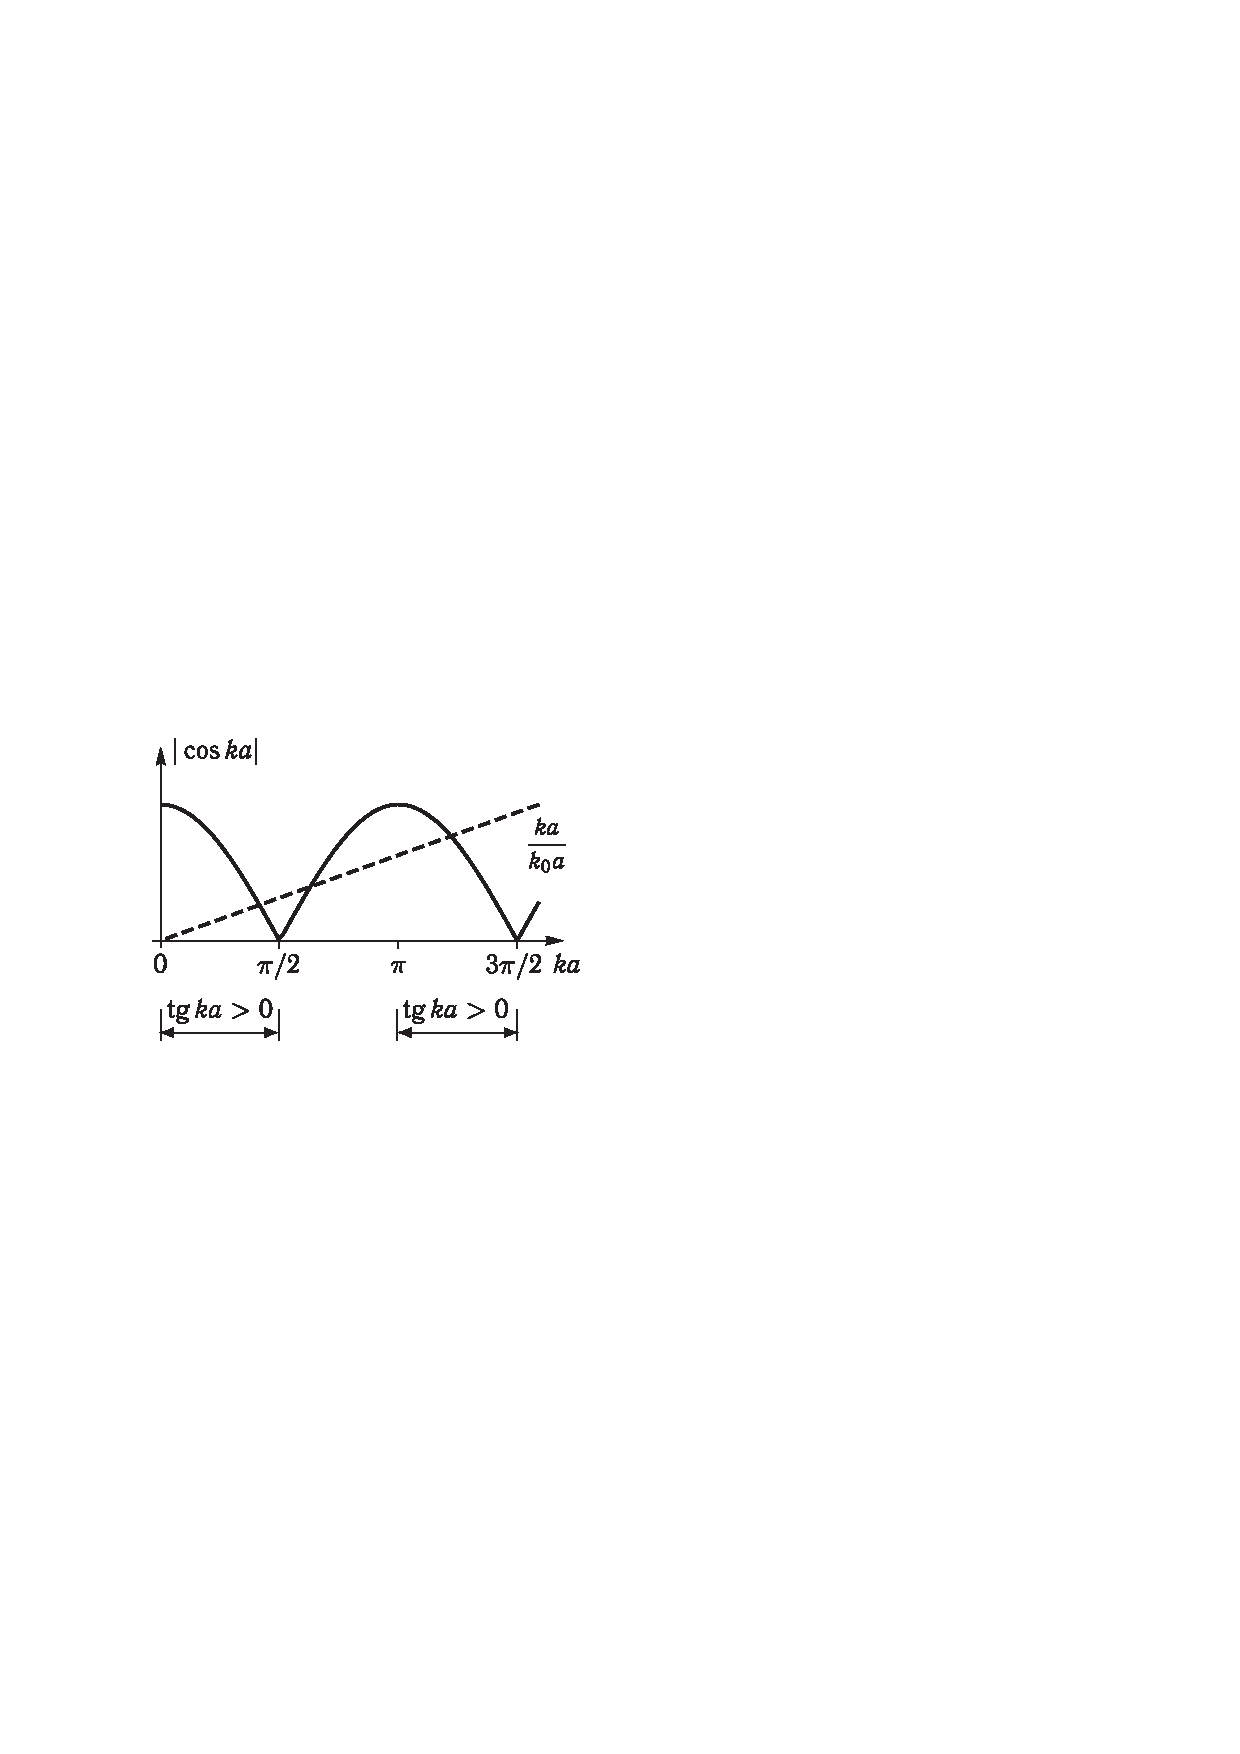
\includegraphics[width=0.5\textwidth]{1}
	\caption{Определение уровней энергии для чётных состояний}
	\label{fig:1}
\end{figure}
\begin{figure}[htpb]
	\centering
	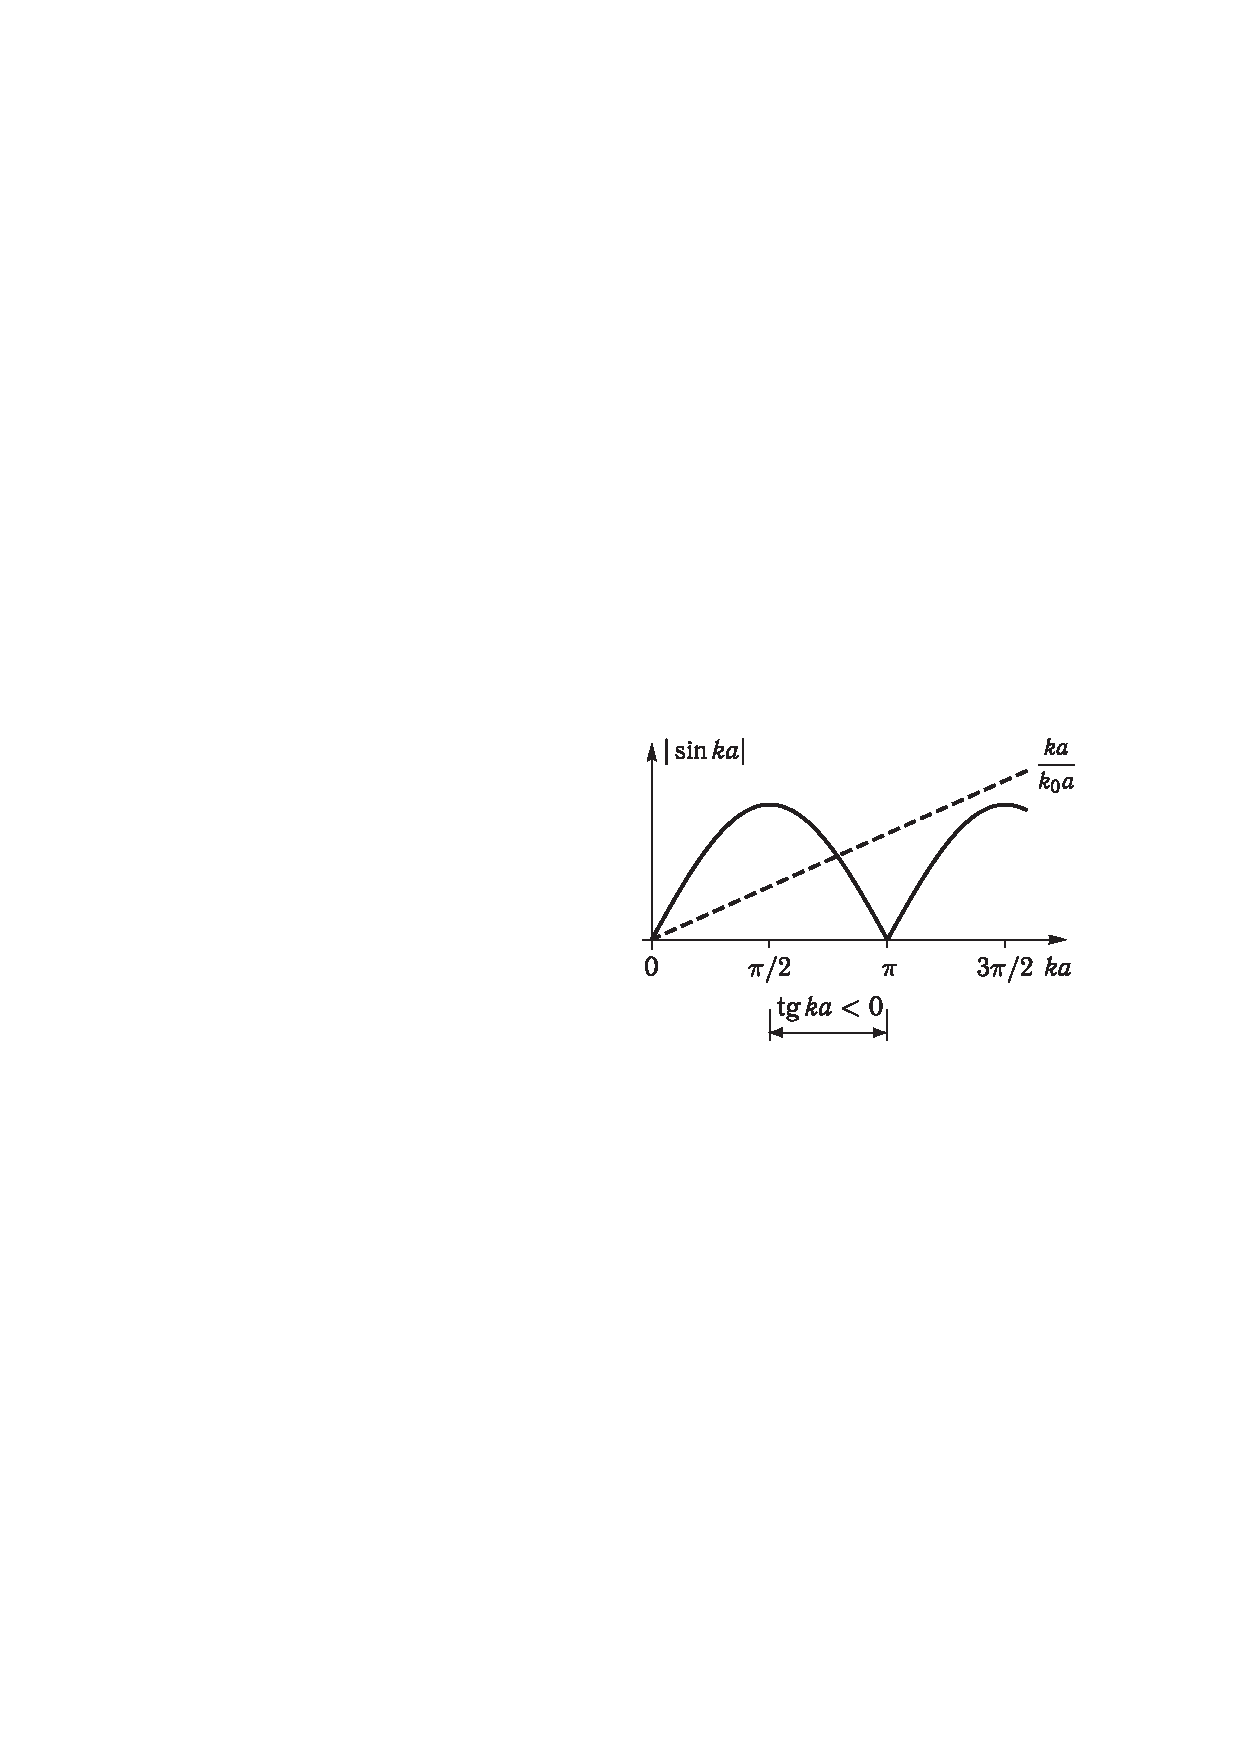
\includegraphics[width=0.5\textwidth]{2}
	\caption{Определение уровней энергии для нечётных состояний}
	\label{fig:2}
\end{figure}

Чётное состояние существует при малой глубине $U_0$ ямы ($k_0 a>0$). $N$ чётных состояний существует при $k_0 a \ge  (N-1) \pi$.
Из условия непрерывности функции
\[
	\psi (a-0)=\psi(a+0)
\] 
получаем
\[
B= A e^{\kappa a} \cos k a
.\] 
Условие нормировки даёт
\[
	1= 2|A|^2 \left( \int\limits_{0}^{a} \cos^2 kx\; dx+
	\int\limits_{a}^{\infty} \cos^2 k a e^{-2 \kappa (x-a)}\; dx \right) ,
\] 
откуда в результате несложных вычислений имеем
\[
	A= \frac{1}{\sqrt{2} } \left( 
	1+ \frac{\sin 2 k a}{2 k a}+ \frac{\cos^2 ka}{\kappa a}\right) ^{-1 /2}, \quad B= A e^{\kappa a} \cos k a
.\] 
Для нечётных состояний волновая функция должна иметь вид
\[
	\psi_E ^{(-)}(x)=
	\begin{cases}
		A \sin kx, & |x|<a,\\
		B \sign (x) e^{-\kappa |x|}, & |x|
		>a,
	\end{cases}
\]
где
\[
	\sign (x)= \begin{cases}
		1,& x>0,\\
		-1,& x<0.
	\end{cases}
\] 
Уровни энергии для нечётных состояний определяются из уравнения
\[
k \ctg ka = - \kappa,\quad k^2 =k_0^2-\kappa^2, \quad \text{т.\:е.
} \quad \left( \frac{k_0}{k} \right) ^2 = 1 + \ctg^2 k a
\]
или
\[
	|\sin ka| = \frac{ka}{k_0 a}\quad \text{при}\quad \tg ka<0
.\] 
Как видно из рис.~\ref{fig:2}, нечётные дискретные состояния
существуют при условии $k_0 a\ge \pi /2$, ($ka / (k_0 a) =1$, когда
$k_0 a = \pi /2$), т.\:е.
\[
U_0 \ge  \frac{\pi^2}{8} \frac{\hbar^2}{m a^2}
.\] 
Это и есть условие существования хотя бы одного нечётного
состояния в такой яме. $N$ нечётных состояний существует при
$k_0 a \ge \pi N /2$.

Из непрерывности функции $\psi(a+0)=\psi(a-0)$ следует
 \[
B= A e^{\kappa a} \sin ka
.\] 
Учитываем условие нормировки нашей функции
\[
	1= 2|A|^2 \left( \int\limits_{0}^{a} \sin^2 kx\; dx+
	\sin^2 ka \int\limits_{a}^{\infty}e^{-2\kappa (x-a)}\;dx
\right) 
\]
и получаем итоговый результат
\[
	A= \frac{1}{\sqrt{a} }\left( 1- \frac{\sin 2 k a}{2ka}+
	\frac{\sin^2 ka}{\kappa a}\right) ^{- 1 / 2},\quad
	B= A e^{\kappa a} \sin ka
.\] 

\item Получим решение задачи о состояниях дискретного спектра
	в данной потенциальной яме на основании анализа
	нечётных решений $\psi^{(-)}_E (x)$ пункта $\ref{item:1}$ данной задачи.

	Граничные условия, накладываемые на волновую функцию в
	точке $x=0$ и на  $\psi$ и $\psi'$ в точке $x=a$.
	Совпадают с соответствующими граничными условиями для
	$\psi^{(-)}_E(x)$. Однако область, где волновая
	функция отлична от нуля уменьшается вдвое. Поэтому
	$\psi^{(-)}_E(x)$ нужно умножить на $\sqrt{2} $. В
	итоге получим волновые функции в виде
	\[
		\psi_E(x)=
		\begin{cases}
			\sqrt{2} \psi^{(-)}_E(x),& x>0,\\
			0,& x\le 0.
		\end{cases}
	\] 
\end{enumerate}
\end{sol}
\begin{problem}
	\label{prob:3}
	\renewcommand{\labelenumi}{\asbuk{enumi})}
	\begin{enumerate}
		\item 
	Найти энергию и волновую функцию связанного состояния
	частицы в поле
	\[
		U(x)= - \frac{\hbar^2\kappa_0}{m}\delta(x)
	.\] 
	Вычислить средние и дисперсии координаты и импульса в
	связанном состоянии.
	\item Найти коэффициенты прохождения и отражения.
	\item Вычислить вероятность <<ионизации>> связанного
		состояния при мгновенном изменения параметра
		глубины ямы с $\kappa_0$ до $\kappa_1$.
	\end{enumerate}
\end{problem}
\begin{sol}
\renewcommand{\labelenumi}{\asbuk{enumi})}
\begin{enumerate}
\item Полагая $E<0$ и вводя обозначение
	\[
	\kappa^2= \frac{2 m |E|}{\hbar^2}
	,\]
получаем уравнение, которому удовлетворяет волновая функция
дискретного невырожденного спектра частицы в виде
\begin{equation}
	\psi''(x)-\left( \kappa^2 - 2\kappa_0 \delta(x) \right) 
	\psi(x)=0
	\label{eq:2}
.\end{equation} 
В точке разрыва потенциала $x=0$ потребуем непрерывности
$\psi(x)$:
\[
	\psi(+0)=\psi(-0)
.\] 
При этом производная $\psi'(x)$ терпит разрыв, величину которого
находим из уравнения \eqref{eq:2}, интегрируя его в пределах
от $-\epsilon $ до $\epsilon$ при $\epsilon \to 0$:
\begin{equation}
	\psi'(+0)-\psi'(-0)=-2\kappa_0 \psi (0)
	\label{eq:3}
.\end{equation}
При этом, как и должно быть, выполняется условие непрерывности
плотности потока вероятности: $j(+0)=j(-0)$, где
\[
	j(x)= \frac{i\hbar }{2m} \left( \psi(x)\psi'(x)^*-
	\psi^*(x)\psi'(x)\right) 
.\] 
Нормированное решение ищем в виде
\[
	\psi(x)= 
	\begin{cases}
		C_1 e^{-\kappa x},& x>0,\\
		C_2 e^{\kappa x},& x<0.
	\end{cases}
\]
Из непрерывности $\psi$ при $x=0$, получаем $C_1=C_2=C$. Тогда
условие  \eqref{eq:3} даёт $\kappa=\kappa_0$, т.\:е.
при $E<0$ имеем всего один дискретный уровень с энергией
\[
E_0= -\frac{\hbar^2 \kappa_0^2}{2m}
\]
и волновой функцией
\[
	\psi_0(x)= \sqrt{\kappa_0} e^{-\kappa_0 |x|}\equiv
	\braket{x|0}
 ,\]
нормированной на единицу.

В импульсном представлении волновая функция найденного дискретного
уровня будет иметь вид
\begin{multline*}
	\psi_0(p)\equiv \braket{p|0}= \int\limits_{-\infty}^{\infty} 
	dx \braket{p|x}
	\braket{x|0}=\\=
	\frac{\sqrt{\kappa_0} }{(2\pi \hbar)^{1 /2}}
	\int\limits_{-\infty}^{\infty} 
	e^{-\kappa_0 |x|- \frac{i p x}{\hbar}}dx=
	\sqrt{\frac{2}{\pi}} \frac{(x_0 \hbar)^3 /2}{(\kappa_0
	\hbar)^2+p^2}
.\end{multline*}
Легко найти $\bra{0}\widehat{\operatorname{x}}\ket{0}=0$,
$\bra{0}\widehat{\operatorname{p}}\ket{0}=0$, а также
\begin{multline*}
\bra{0}\widehat{\operatorname{x}}^2\ket{0}
=\int\limits_{-\infty}^{\infty} \kappa e^{-2 \kappa_0 |x|}
\widehat{\operatorname{x}}^2 dx= \alpha \int\limits_{0}^{\infty}
e^{-\alpha x}x^2dx=\\= \alpha \frac{d^2}{d\alpha^2}
\int\limits_{0}^{\infty} e^{-\alpha x}dx= \left. 
	\frac{2}{\alpha^2}\right|_{\alpha=2\kappa_0}=\frac{1}{
	\kappa_0^2} 
,\end{multline*} 
и, кроме того,
\begin{multline*}
\bra{0}\widehat{\operatorname{p}}^2\ket{0}=
\int\limits_{-\infty}^{\infty} dp \, p^2 \frac{2}{\pi}
\frac{(\kappa_0\hbar)^3}{\left( (\hbar\kappa_0)^2+p^2 \right) ^2}=
\frac{2}{\pi} (\kappa_0 \hbar)^3 \left( - \frac{d}{d\alpha^2} \right) \int\limits_{-\infty}^{\infty} \frac{p^2 dp}{\alpha^2+p^2}=
\\=\frac{2}{\pi} (\kappa_0 \hbar)^3 \left( -\frac{d}{d\alpha^2} \right) \left. \frac{2\pi i (i\alpha)^2}{2i \alpha} \right|_{\alpha
	=\kappa\hbar}=(\kappa_0\hbar)^2
.\end{multline*} 
Откуда находим дисперсии
\[
	\left(\Delta \widehat{\operatorname{x}}\right)^2=
	\bra{0}\widehat{\operatorname{x}}^2\ket{0}-
	\bra{0}\widehat{\operatorname{x}}\ket{0}^2=
	\frac{1}{\kappa_0^2}
 ,\] 
\[
	\left(\Delta \widehat{\operatorname{p}}\right)^2=
	\bra{0}\widehat{\operatorname{p}}^2\ket{0}-
	\bra{0}\widehat{\operatorname{p}}\ket{0}^2=
	(\kappa_0 \hbar)^2
.\] 
\item Волновая функция частицы массы $m$, свободно двигавшейся вдоль оси $x$ с энергией $E>0$ и попавшей в область действия $\delta$-потенциала будет иметь вид
\[
	\psi(x)= \begin{cases}
		e^{i\kappa x}+A e^{-i\kappa x},& x<0,\\
		Be^{i \kappa x},& x>0
	\end{cases}
,\]
где, как и ранее,
\[
\kappa^2=\frac{2m E}{\hbar^2}
 .\] 
Запишем уравнение Шрёдингера
\begin{equation}
	\psi''(x)+\left(\kappa^2+2\kappa_0 \delta(x)\right)
	\psi(x)=0
	\label{eq:4}
.\end{equation} 
Как и в предыдущем пункте в точке разрыва потенциала $x=0$ 
потребуем  непрерывности $\psi(x)$:
 \[
	 \psi(+0)=\psi(-0)
.\] 
При этом производная $\psi'(x)$ терпит разрыв, величину которого
находим из уравнения \eqref{eq:4}, интегрируя его в пределах
от $-\epsilon $ до $\epsilon $ при $\epsilon\to 0$:
\begin{equation}
	\psi'(+0)-\psi'(-0)=-2\kappa_0 \psi(0)
	\label{eq:5}
.\end{equation} 
При этом, как и ранее, выполняется условие непрерывности
плотности потока вероятности $j(+0)=j(-0)$, где
 \[
	 j(x)= \frac{i \hbar }{2m} \left( \psi(x)
	 \psi'(x)^*-\psi^*(x)\psi'(x)\right) 
.\] 
Из непрерывности при $x=0$ получаем $1+A=B$. Тогда условие 
 \eqref{eq:5} даёт
 \[
A= \frac{-\kappa_0}{i\kappa+\kappa_0}
 .\] 
Откуда
\[
R= \frac{|j_\text{отр}|}{|j_{\text{пад}}|}=|A|^2=
\frac{\kappa_0^2}{\kappa^2+\kappa_0^2},\quad
D=\frac{|j_{\text{прош}}|}{|j_\text{пад}|}=|B|^2=
\frac{\kappa^2}{\kappa^2+\kappa_0^2}
.\] 
Очевидно, что выполняется равенство $D+R=1$. 
\item Изначально
\[
	\psi(x)= \sqrt{\kappa_0} e^{-\kappa_0 |x|}
,\]
после резкого изменения параметра $\kappa$ связанное состояние
частицы описывается функцией
\[
	\phi(x)= \sqrt{\kappa_1} e^{-\kappa_1 |x|}
.\]
Вероятность оказаться в состоянии $\phi$
 \[
	 W_\text{ост}=|\braket{\phi|\psi}|^2=
	 \left( \sqrt{\kappa_0 \kappa_1}\cdot_2 \int\limits_{0}
	 ^{\infty} e^{-(\kappa_0+\kappa_1)x}dx  \right) ^2=
	 \frac{4\kappa_0^2 \kappa_1^2}{(\kappa_0+\kappa_1)^2}
.\] 
Вероятность вылететь из ямы (<<ионизации>>):
\[
	W_i=1- \frac{4\kappa_0^2 \kappa_1^2}{(\kappa_0+\kappa_1)^2}=\frac{(\kappa_0-\kappa_1)^2}{(\kappa_0+\kappa_1)^2}
.\] 
\end{enumerate}
\end{sol}
\begin{problem}
	Найти коэффициенты прохождения и отражения частицы
	\renewcommand{\labelenumi}{\asbuk{enumi})}
	\begin{enumerate}
		\item на прямоугольном  потенциальном барьере,
		\item на прямоугольной потенциальной яме.
	\end{enumerate}
\end{problem}
\begin{sol}
		При рассмотрении задачи о нахождении коэффициентов отражения
и прохождения мы будем исходить из потенциала
\[
	U(x)= \begin{cases}
		-U_0,& |x|<a /2,\\
		0,& |x|
		>a /2.
	\end{cases}
\]

Волновая функция частицы будет иметь вид
\[
	\psi(x)= 
	\begin{cases}
		e^{ikx}+ A e^{-ikx},& x< a /2,\\
		C e^{i k_1 x}+ D e^{- i k_1 x},& |x|< a /2,\\
		Be^{ikx},& x>a /2,
	\end{cases}
\] 
где
\[
	k^2= \frac{2mE}{\hbar^2}>0,\quad k_1^2 = \frac{2 m (E+U_0)}{\hbar^2}
.\] 

Учёт условий непрерывности волновой функции $\psi$ и её производной
$\psi'$ в точках $x=\pm a /2$ даёт систему из четырёх уравнений.
В результате решения этой системы имеем
\[
	A= \frac{i e^{-ika}\left( k_1^2-k^2 \right) \sin k_1a}{
	2kk_1 \cos k_1 a - i \left( k_1^2 +k^2 \right) \sin k_1 a}
 ,\] 
\[
	B= \frac{2 k k_1 e^{-i k_1 a}}{2 k k_1 \cos k_1 a- i \left( 
	k_1^2+k^2\right) \sin k_1 a}
.\] 
Таким образом, для коэффициента отражения получаем
\begin{multline*}
R= \frac{|j_x^\text{отр}|}{|j_x^\text{пад}|}= |A|^2=
\frac{\left(k_1^2-k^2\right)\sin^2 k_1 a}{4 k_1^2 k^2 \cos^2 k_1 a+
\left( k_1^2+k^2 \right) ^2 \sin^2 k_1 a}=\\= \frac{
\left( k_1^2-k^2 \right)\sin^2 k_1 a }{4k_1^2 k^2 + \left( 
k_1^2-k^2\right) ^2 \sin^2 k_1 a}
.\end{multline*} 
Величина $R$ обращается в ноль при $k_1 a = \frac{a}{\hbar }\sqrt{
2 m (E+U_0)} =n \pi,\; n= 1,\,2,\ldots,$ а также, естественно, при
$k=k_1$, ($U_0=0$).

Коэффициент прохождения имеет вид
\begin{multline*}
D= \frac{|j_x^\text{прош}|}{|j_x^\text{пад}|}= |B|^2=
\frac{4k_1^2 k^2}{4 k_1^2 k^2 \cos^2 k_1 a +\left( k_1^2+
k^2\right) ^2 \sin^2 k_1 a}=\\= \frac{4 k_1^2 k^2}{4 k_1^2 k^2+
\left( k_1^2 -k^2 \right) ^2 \sin^2 k_1 a}
.\end{multline*} 
Очевидно, что выполняется равенство $D+R=1$.

Полученные результаты для коэффициентов прохождения и отражения
будут справедливы и в случае потенциального барьера (рис.~\ref{fig:3})
\begin{figure}[htpb]
	\centering
	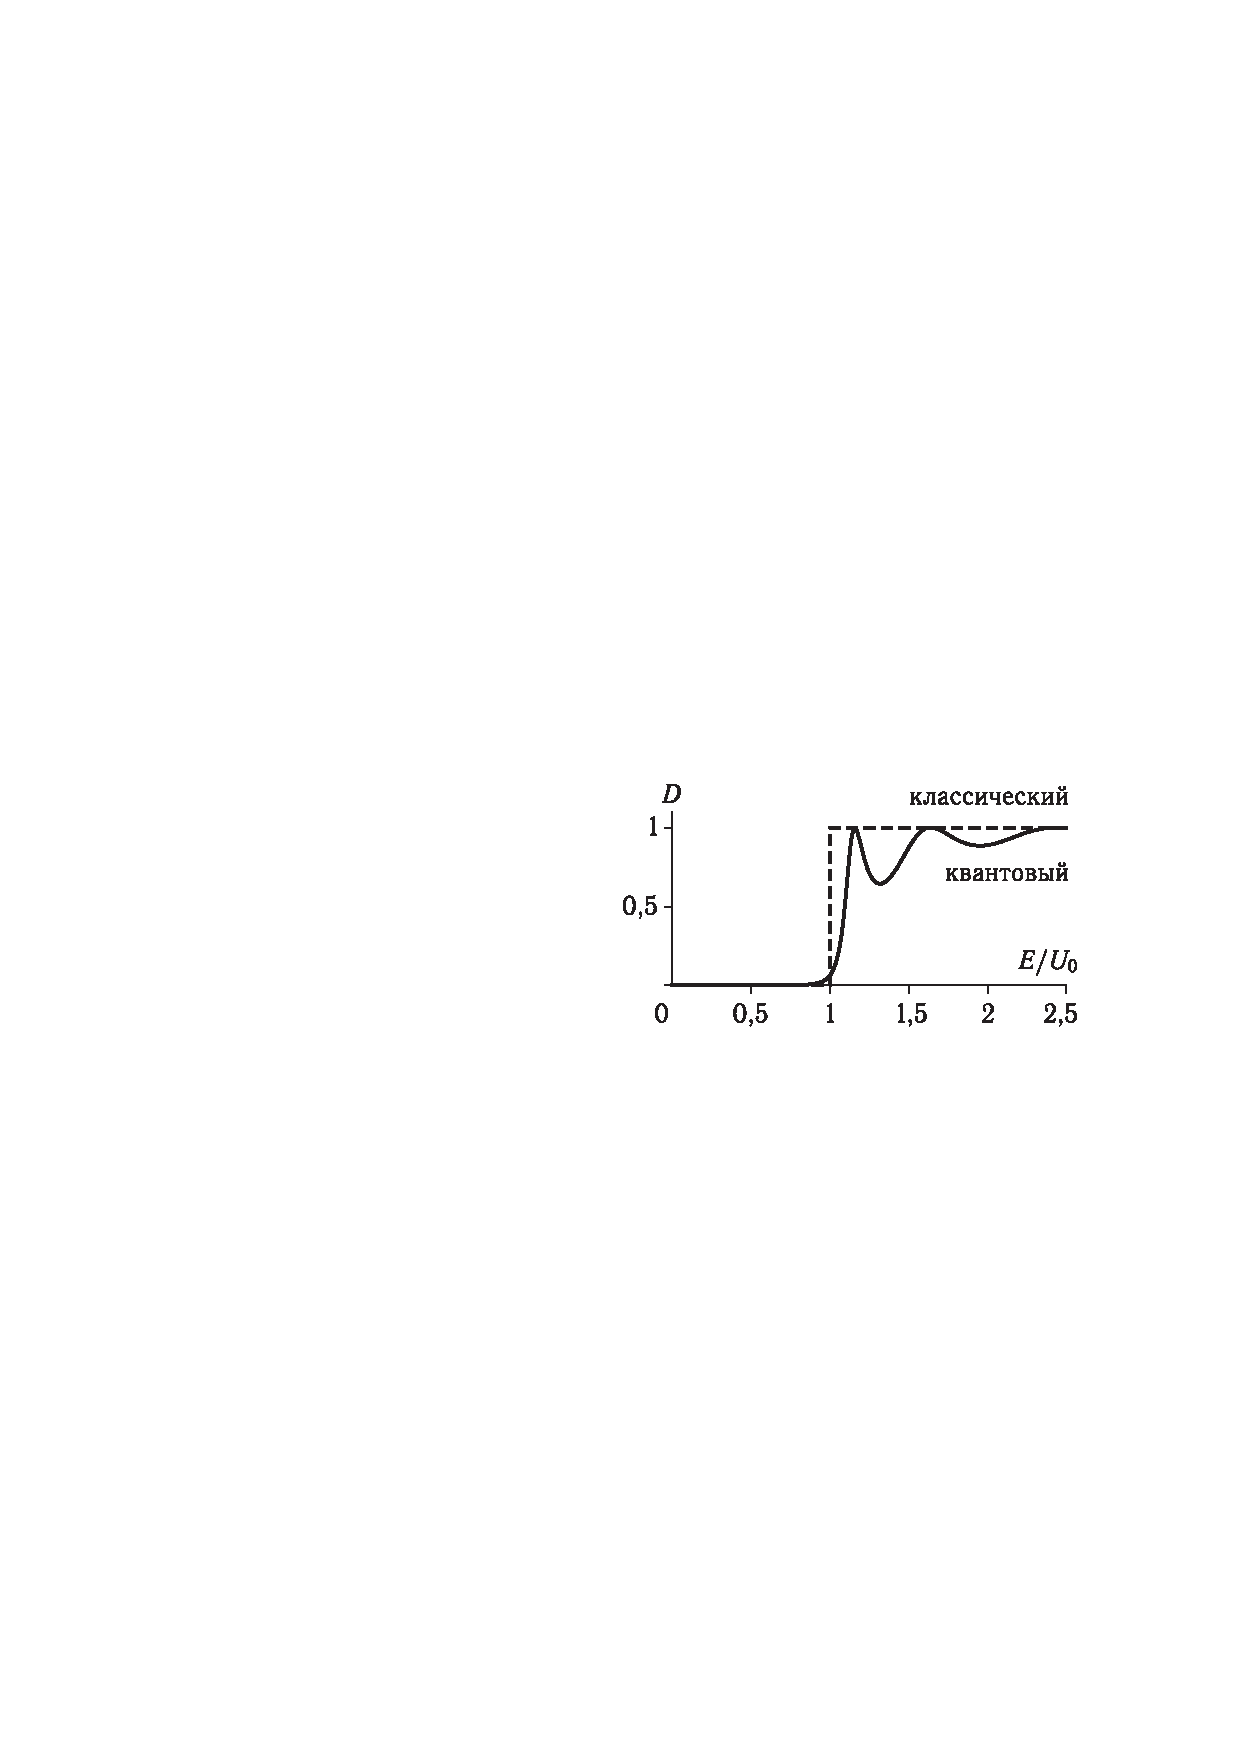
\includegraphics[width=0.5\textwidth]{3}
	\caption{Коэффициент прохождения для потенциального барьера}
	\label{fig:3}
\end{figure}
если в формуле $k_1^2= \frac{2m}{\hbar^2}(E+U_0)$ осуществить замену
$U_0\to -U_0$.

При $0<E<U_0$ нужно дополнительно положить $k_1=i\kappa$, где
$
	\kappa_1^2= \frac{2m}{\hbar^2}(U_0-E)
.$ В результате получаем
\[
	R=\frac{(\kappa^2+k^2) \sh^2 \kappa_1 a}{4 \kappa_1^2 k^2
	+\left( \kappa_1^2 +k^2 \right) ^2 \sh^2 \kappa_1 a}
 ,\]
\[
	D= \frac{4\kappa_1^2 k^2}{4\kappa_1^2 k^2 + (\kappa_1^2+
	k^2)^2 \sh^2 \kappa_1 a}
.\] 
Из рис.~\ref{fig:3} видно, что коэффициент прохождения $D$ в квантовом
случае достигает максимального значения $D=1$ (классический предел)
лишь при $k_1 a=\pi n$, $n=1,\,2,\ldots$. Между этими максимумами
находятся минимумы, причём значение $D$ в этих точках растёт с
ростом величины $E /U_0$. Данные отличия в поведении квантового
коэффициента прохождения от классического связаны с проявлением
волновых свойств частиц.
\end{sol}
\begin{problem}
	Найти уровни энергии и волновые функции связанных состояний частицы в поле
\[
	U(x)= - \frac{\hbar^2 \kappa_0}{m}\left\{ 
	\delta(x+a)+\delta(x-a)\right\} 
.\] 
Рассмотреть предел $\kappa_0 a \gg 1$ и эволюцию начального состояния, отвечающего волновой функции частицы, связанной в одной
яме при $x=-a$, определить вероятность обнаружить частицу в той
же яме в момент времени $t$ и частоту осцилляций.
\end{problem}
\begin{sol}
Очевидно, что данный потенциал представляет собой чётную функцию
$U(-x)=U(x)$, поэтому гамильтониан коммутирует с оператором
инверсии
\[
[ \widehat{\operatorname{H}},\,\hat{\operatorname{I}} ] =0
 ,\] 
и можно искать решение уравнения Шрёдингера, как общие собственные
 функции операторов $\widehat{\operatorname{H}}$ и $\hat{\operatorname{I}}$,
т.\:е. в виде чётных и нечётных функций. Запишем общий вид
чётного и нечётного решения на всей числовой прямой, исключая
сами $\delta$-функции $(E<0,\; \kappa^2 = 2 m |E| /\hbar^2)$ 
\[
	\psi^{(+)}(x) =
	\begin{cases}
		B e^{\kappa x}, & x<-a,\\
		A \ch \kappa x, & -a <x<a,\\
		B e^{-\kappa x},& x>a,
	\end{cases}
\]
\[
	\psi^{(-)}(x)=
	\begin{cases}
		B e^{\kappa x},& x<-a\\
		A \sh \kappa x, & -a<x<a,\\
		-B e^{-\kappa x},& x>a.
	\end{cases}
\]

Учитываем условия <<сшивания>> решений: непрерывность функции
при $x=a$ 
\begin{equation}
	\psi(a+0)=\psi(a-0)
	\label{eq:291}
\end{equation} 
и конечный разрыв производной (как и в задаче \ref{prob:3})
\begin{equation}
	\psi'(a+0)-\psi'(a-0)=-2\kappa_0 \psi (a)
	\label{eq:52}
.\end{equation} 

Условие совместности уравнений \eqref{eq:291} и \eqref{eq:52}
с учётом явного вида $\psi^{(+)}(x)$ и $\psi^{(-)}(x)$ даёт
трансцендентное уравнение для нахождения уровней энергии
\begin{equation}
\frac{\kappa a}{\kappa_0 a}=1 \pm e^{-2\kappa a}
\label{eq:53}
 ,\end{equation}
где верхний знак отвечает чётному, а нижний --- нечётному
уровню энергии.

Анализ уравнения \eqref{eq:53} показывает (рис.~\ref{fig:4}),
\begin{figure}[htpb]
	\centering
	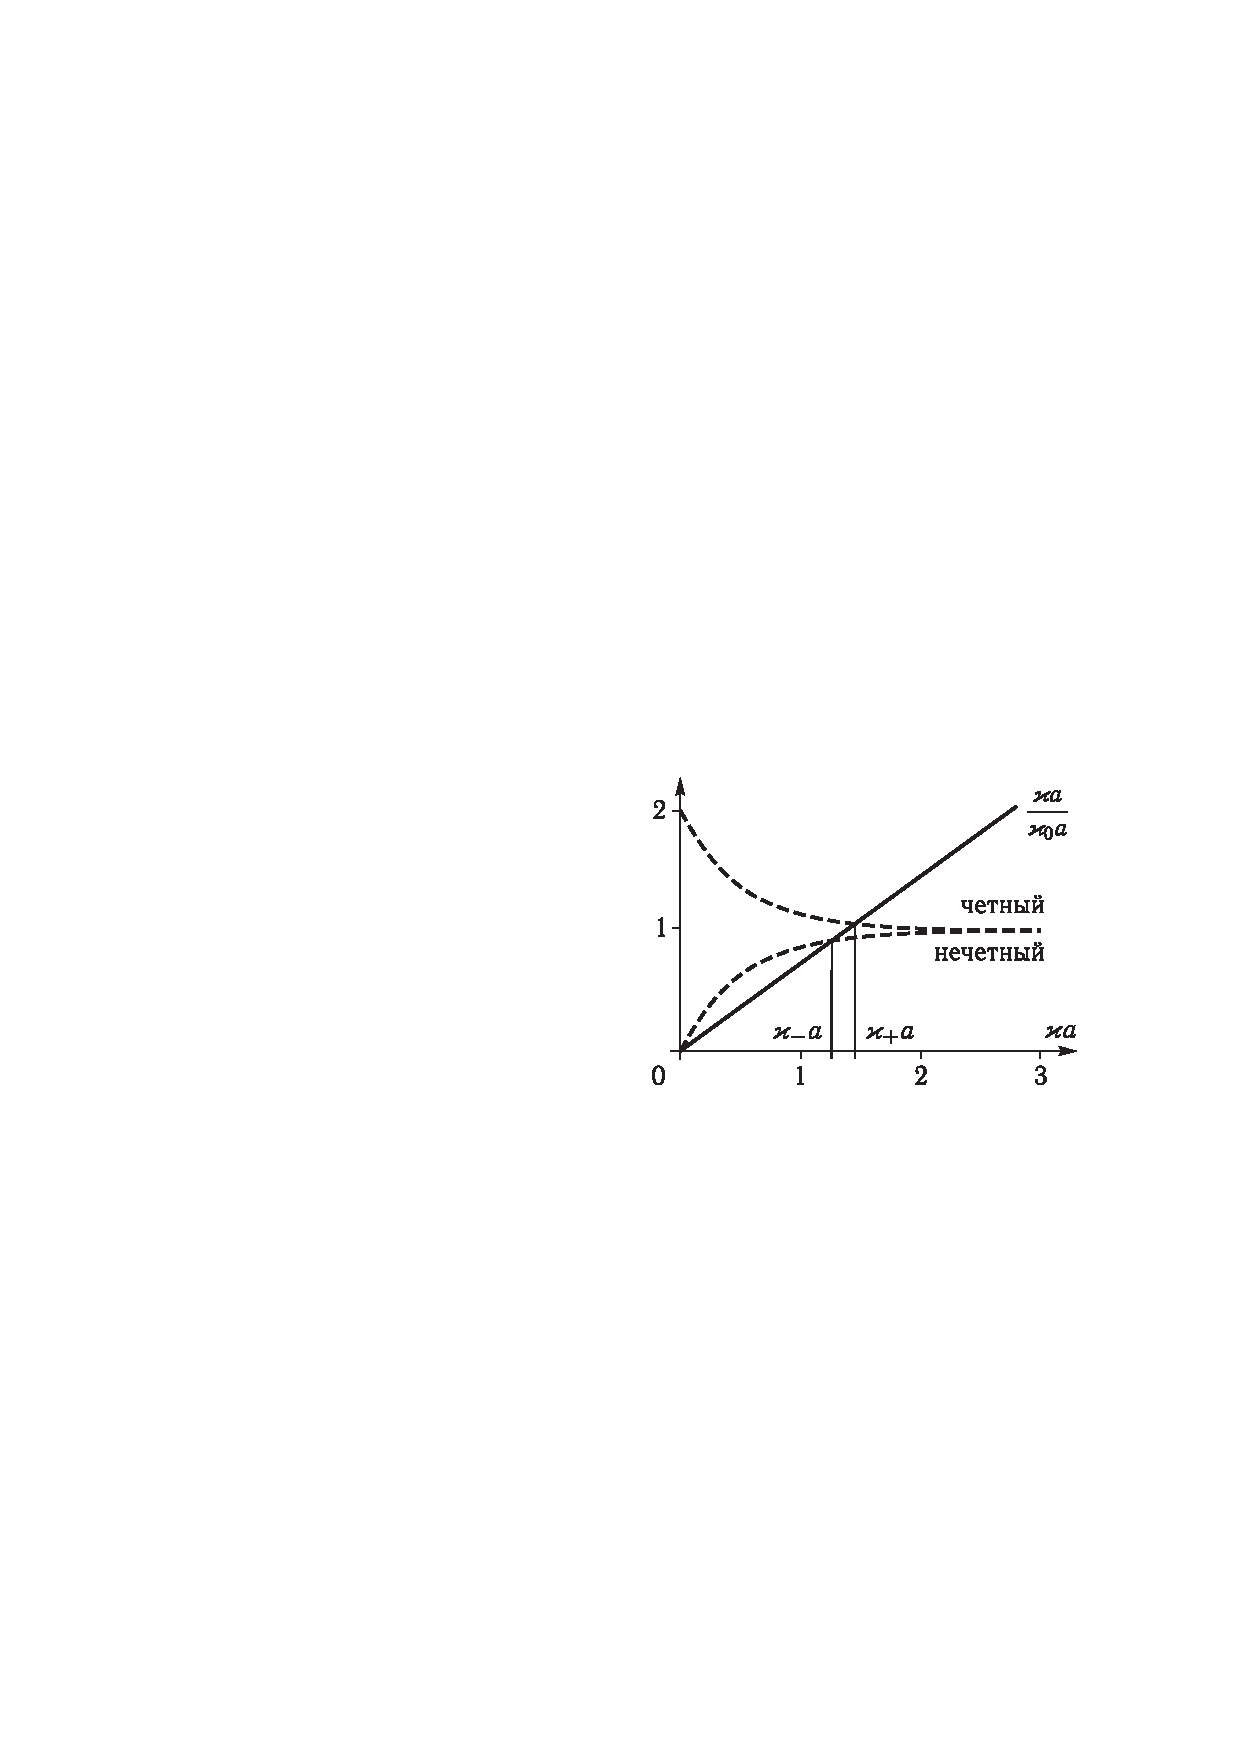
\includegraphics[width=0.5\textwidth]{4}
	\caption{Графический анализ уравнения \eqref{eq:53}}
	\label{fig:4}
\end{figure}
что в данном потенциале в общем  случае существуют два
дискретных уровня энергии --- чётный и нечётный. Чётный уровень
лежит ниже и присутствует всегда, нечётный лежит выше и
существует только при $\kappa_0 a \ge  1 /2$. Таким образом,
при малых расстояниях между ямами остаётся только чётный уровень.

Если $\kappa a \ll 1$, то $\kappa \simeq 2 \kappa_0$ и энергия
чётного состояния
\[
E^{(+)}= -4 \frac{\hbar^2 \kappa_0^2}{2m}
 ,\]
т.\:е. при малом расстоянии две $\delta$-ямы действуют, как одна,
но с удвоенным значением $\kappa_0$. Если же ямы далеки друг
от друга (при $\kappa_0 a \gg 1$ ), то уровни энергии
экспоненциально мало отличаются друг от друга и в конце концов
сливаются. В результате мы получаем задачу о двух $\delta$-ямах,
независимых друг от друга.

Находим нормировочные коэффициенты для чётной и нечётной волновых
функций
\[
	A^{(+)}= \frac{1}{\sqrt{a} } \left( 1+
	\frac{\sh 2\kappa a}{2 \kappa a}+ \frac{\ch^2 \kappa a}{\kappa a}\right) ^{- 1 /2}, \quad B^{(+)}= A^{(+)}e^{\kappa a}
	\ch \kappa a
 ,\]
\[
	A^{(-)}=\frac{1}{\sqrt{a} }\left( -1+
	\frac{\sh 2 \kappa a}{2\kappa a}+ \frac{\sh^2 \kappa a}{
\kappa a}\right) ^{- 1 /2},\quad B^{(-)}=A^{(-)} e^{\kappa a}
\sh \kappa a
.\] 
При исследовании задачи эволюции начального состояния, отвечающего
 волновой функции частицы, связанной в одной яме при $x=-a$,
используем следующие предположения
\renewcommand{\labelenumi}{\asbuk{enumi})}
\begin{enumerate}
	\item $\delta$-ямы находятся достаточно далеко друг
		от друга, т.\:е. в системе ям имеется два
		дискретных уровня энергии, отвечающих
		связанным состояниям. Однако ямы не бесконечно
		далеки, следовательно, $E^{(+)}\neq E^{(-)}$.
	\item Система, рассматриваемая нами, --- приближенно
		двухуровневая, т.\:е. отброшен весь непрерывный
		спектр --- считается, что частица не выходит
		из ям.
\end{enumerate}
Как это следует из рис.~\ref{fig:5},
\begin{figure}[htpb]
	\centering
	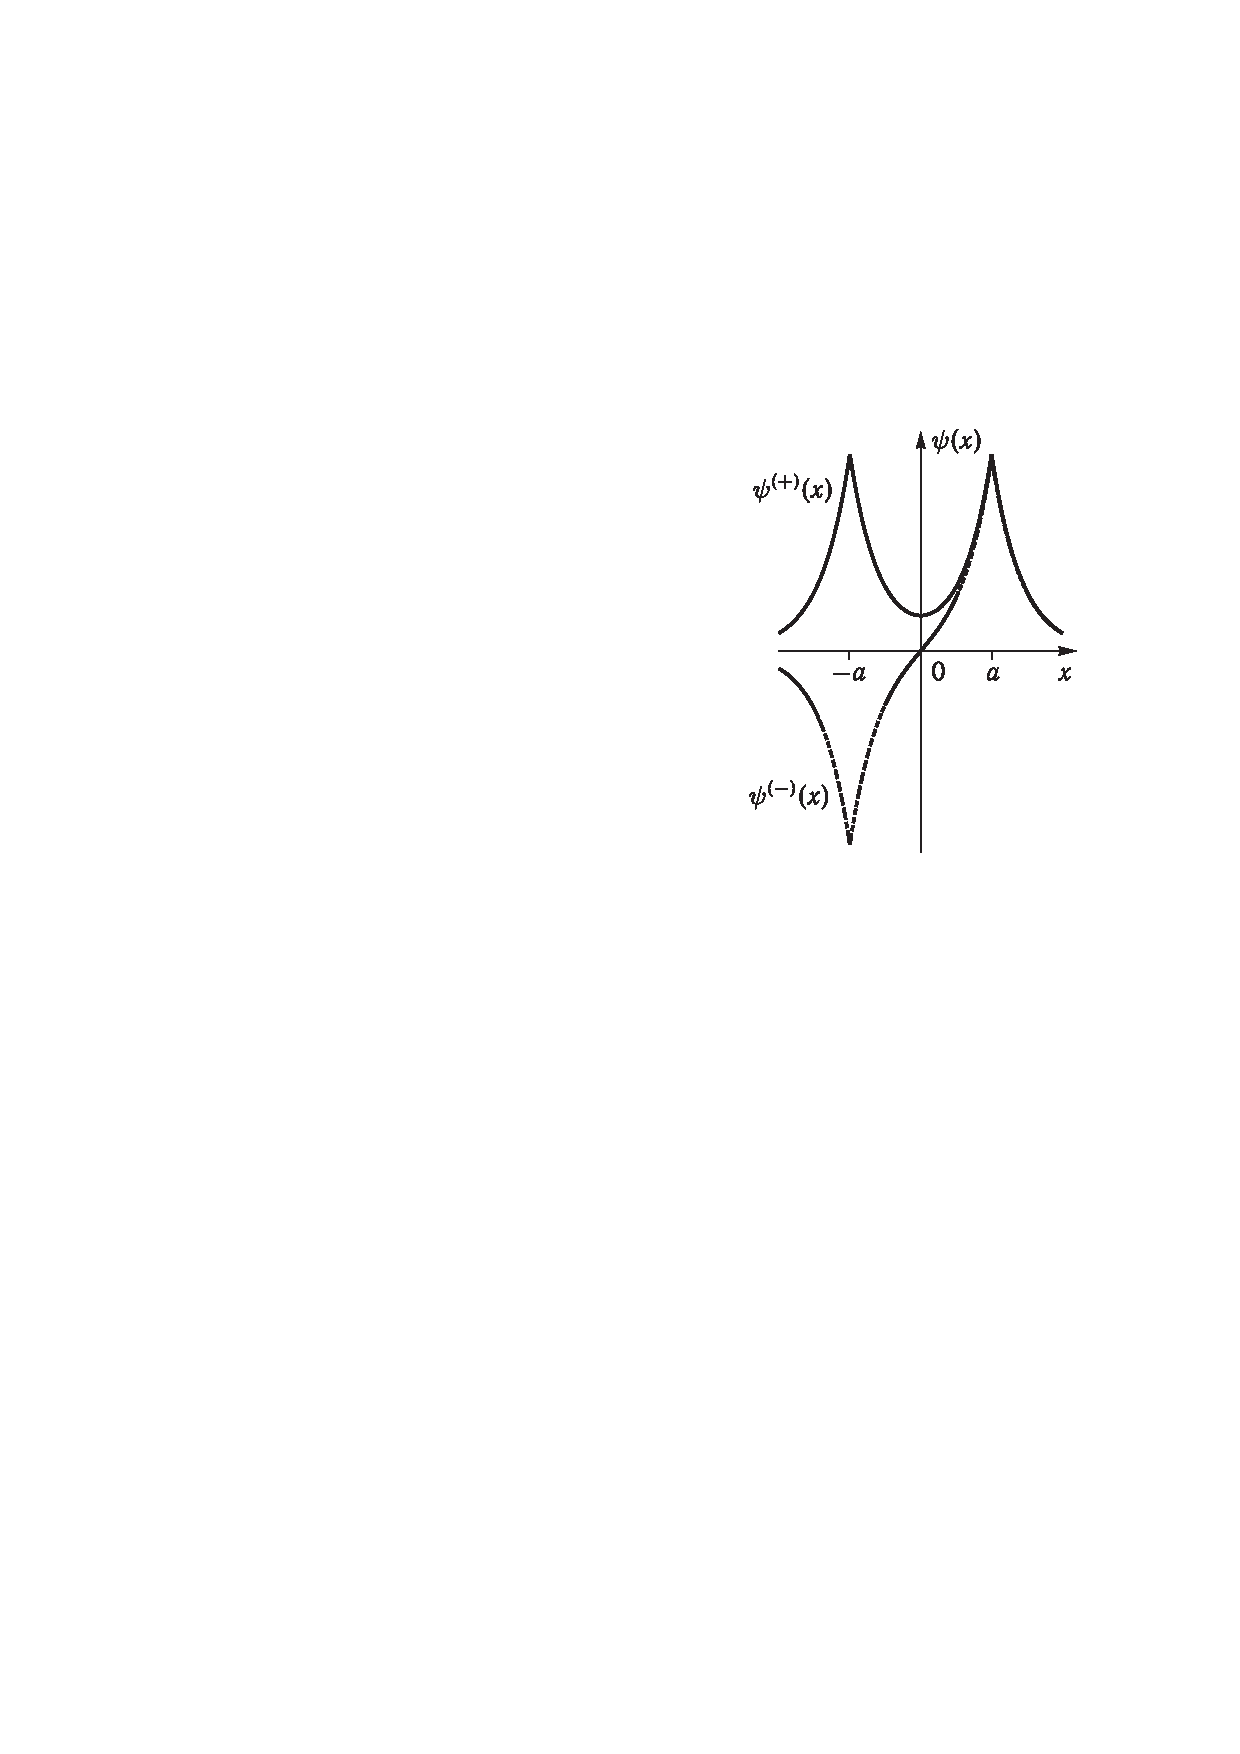
\includegraphics[width=0.4\textwidth]{5}
	\caption{Стационарные состояния для системы двух
	$\delta$-ям}
	\label{fig:5}
\end{figure}
в любом из \emph{стационарных} состояний $\psi^{(+)}(x)$ или
$\psi^{(-)}(x)$ выполняется
\[
	\left| \psi^{(\pm)}(-x) \right| ^2= \left| 
	\psi^{(\pm)}(x)\right| ^2
 ,\]
поэтому вероятность обнаружения частицы вблизи левой и правой
ямы одинакова --- частица не локализована вблизи ни одной из
ям.

С целью построить состояние, в котором частица (хотя бы в начальный
момент времени) была бы локализована в окрестности одной из ям,
воспользуемся линейной комбинацией функций
\begin{equation}
	\Psi(x,\,t)= C_1 e^{- \frac{i E^{(+)}t}{\hbar }}
	\psi^{(+)}(x) +C_2 e^{- \frac{i E^{(-)}t}{\hbar }}\psi^{(-)}(x)
\label{eq:521}
.\end{equation}
Очевидно, что в начальный момент времени
\[
	\Psi(x,\,0)=C_1 \psi^{(+)}(x)+C_2 \psi^{(-)}(x)
.\] 
Если положить $C_1=C_2$, то мы получим состояние (рис.~\ref{fig:5}), в котором частица локализована вблизи правой $\delta$-ямы.
Обозначим это состояние $\Psi(x,\,0)=\psi_a(x)$. По аналогии
можно построить состояние $\psi_{-a}(x)$ с локализацией частицы
вблизи левой $\delta$-ямы. Окончательно
\[
\left\{
\begin{aligned}
	\psi_a(x)&= \frac{1}{\sqrt{2} }\left( \psi^{(+)}(x)+
	\psi^{(-)}(x)\right) ,\\
		\psi_{-a}(x)&= \frac{1}{\sqrt{2} }\left( \psi^{(+)}(x)-
	\psi^{(-)}(x)\right),
\end{aligned}
\right.
\]
и обратно
\[
\left\{
\begin{aligned}
	\psi^{(+)}(x)&= \frac{1}{\sqrt{2} }\left( \psi_a (x)+
	\psi_{-a}(x)\right),\\
		\psi^{(-)}(x)&= \frac{1}{\sqrt{2} }\left( \psi_a(x)-
	\psi_{-a}(x)\right) 
\end{aligned}
\right.
.\] 
Итак, волновая функция \eqref{eq:521}, в котором частица в
начальный момент времени локализована вблизи правой $\delta$-ямы,
имеет вид
\begin{multline*}
	\Psi(x,\,t)= \frac{1}{\sqrt{2} }\left\{ e^{- \frac{i E
	^{(+)}t}{\hbar }}\psi^{(+)}(x)+e^{- \frac{i E^{(-)}t}{\hbar }}\psi^{(-)}(x) \right\} =\\=
	\frac{1}{2}\left\{ \psi_a(x) \left[ 
	e^{- \frac{i E^{(+)}t}{\hbar }}+ e ^{- \frac{i E^{(-)}t}{
	\hbar }}\right] +\psi_{-a}(x) \left[ e^{- \frac{i E^{(+)}
	t}{\hbar }}- e^{-\frac{i e^{(-)}t}{\hbar }} \right]  \right\} 
.\end{multline*} 

В соответствии со статистической интерпретацией, вероятность обнаружить
частицу локализованной вблизи левой ямы, если в начальный момент
она была локализована в правой, равна
\begin{multline*}
W_{-a}= \frac{1}{4} \left| e^{- \frac{i E^{(+)}t}{\hbar }}-
e^{- \frac{i E^{(-)}t}{\hbar }}\right| ^2= \frac{1}{2}\left[ 
1- \cos \left( \frac{E^{(+)}-E^{(-)}}{\hbar }t \right) \right] =\\=
\sin^2 \left[ \frac{E^{(+)}-E^{(-)}}{2\hbar }t \right] 
.\end{multline*} 
\end{sol}
\begin{problem}
	Найти волновую функцию, минимизирующую соотношение неопределённостей для координаты и импульса:
	\[
	\Delta x\cdot \Delta p= \frac{\hbar }{2}
	.\] 

\end{problem}
\begin{sol}
Как известно, коммутатор $[\widehat{\operatorname{p}},\,
\widehat{\operatorname{x}}]=i\hbar \widehat{\operatorname{\mathbb{1}}}$
Пусть
\[
\left\{
\begin{aligned}
	\left< \widehat{\operatorname{p}} \right> &= \bra{\psi} \widehat{\operatorname{p}}\ket{\psi},\\
		\left<\widehat{\operatorname{x}} \right> &=
	\bra{\psi}\widehat{\operatorname{x}}\ket{\psi},
\end{aligned}
\right.
 \quad \text{и тогда}\quad
 \left\{
 \begin{aligned}
	 \Delta \widehat{\operatorname{p}}&=\widehat{\operatorname{p}}-
 \left< \widehat{\operatorname{p}} \right> \widehat{\operatorname{\mathbb{1}}},\\
	 \Delta \widehat{\operatorname{x}}&=\widehat{\operatorname{x}}-
 \left<\widehat{\operatorname{x}} \right>\widehat{\operatorname{
 \mathbb{1}}},
 \end{aligned}
 \right.\] 
при этом, очевидно $[\Delta \widehat{\operatorname{p}},\,
\Delta \widehat{\operatorname{x}}]=i \hbar \widehat{\operatorname{
 \mathbb{1}}}$. Введём в рассмотрение вектор $\ket{\phi}$ 
такой, что
\[
	\ket{\phi}= (\Delta \widehat{\operatorname{p}}-i \gamma
	\Delta \widehat{\operatorname{x}})\ket{\psi}
 , \quad \text{тогда}\quad
 \bra{\phi}= \bra{\psi} (\Delta \widehat{\operatorname{p}}+i
 \gamma \Delta \widehat{\operatorname{x}}).\] 
Здесь мы учли эрмитовость операторов, действительность средних
значений, а также $\gamma^*=\gamma$ по определению. Построим
следующую конструкцию:
\begin{multline*}
\braket{\phi|\phi}=\| 
\ket{\phi}\|^2= \bra{\psi} (\Delta \widehat{\operatorname{p}}+
i \gamma \Delta \widehat{\operatorname{x}})(\Delta
\widehat{\operatorname{p}}- i \gamma  \Delta \widehat{\operatorname{x}})\ket{\psi}=\\=
\left<(\Delta \widehat{\operatorname{p}})^2 \right>+\gamma^2
\left<(\Delta \widehat{\operatorname{x}})^2 \right>+\gamma \hbar
 \ge 0
 ,\end{multline*} 
ибо квадрат нормы вектора положительно определён. По определению дисперсии
\[
	(\Delta p)^2=\left<(\Delta \widehat{\operatorname{p}})^2 \right>
,\]
\[
	(\Delta x)^2=\left<(\Delta \widehat{\operatorname{x}})^2 \right>
,\]
Мы получили
квадратный трёхчлен относительно $\gamma$. Для того, чтобы это
выражение было положительным, нужно, чтобы его дискриминант
$D \le 0$, т.\:е.
\[
	\hbar^2 - 4 (\Delta p)^2
	(\Delta x)^2 \le 0
.\] 
Мы получили соотношение неопределённостей
\[
	\Delta x\cdot\Delta p \ge  \frac{\hbar}{2}
.\] 
Очевидно, что оно минимизируется если детерминант равен нулю
и существует единственный вещественный корень для параметра
$\gamma=\zeta \in \mathbb{R}$. При этом значении параметра
составленный нами вектор состояния $\ket{\phi}$ имеет нулевую
норму, а значит, и сам  он равен нулю, $\ket{\phi}=0$, т.\:е.
\[
	(\Delta \widehat{\operatorname{p}}-i \zeta 
	\Delta \widehat{\operatorname{x}})\ket{\psi}=0
	\Leftrightarrow 
	( \widehat{\operatorname{p}}- \left< \widehat{\operatorname{p}} \right>) \ket{\psi}= i \zeta
		(\widehat{\operatorname{x}}-\left<
		\widehat{\operatorname{x}}\right>)\ket{\psi},
		\quad \zeta \in \mathbb{R}
.\] 
Равенство нулю детерминанта определяет значение $\zeta$, так как
уравнение принимает вид
\[
	\hbar^2 \gamma^2 +4 (\Delta p)^2 \gamma \hbar+4 (\Delta p)^4=0
\] 
с единственным корнем
\[
	\zeta= - 2 \frac{(\Delta p)^2}{\hbar}\implies
	|\zeta|= \frac{\Delta p}{\Delta x}
.\] 
В координатном представлении получаем
\[
	\left(x- \left<\widehat{\operatorname{x}} \right>\right)
	\psi(x) = i \zeta \left( - i \hbar \frac{d}{dx}-
	\left<\widehat{\operatorname{p}} \right>\right) \psi(x)
.\] 
Мы можем переписать это как
\[
	\zeta \frac{d}{dx}\psi (x) - x \psi(x) +\left( 
	\left<\widehat{\operatorname{x}} \right>- i \zeta 
\left<\widehat{\operatorname{p}} \right>\right) \psi(x)
.\] 
Далее упростим:
\[
	\zeta \hbar \frac{d}{dx} \psi= \psi \left(x- \left<\widehat{\operatorname{x}} \right>+i \zeta \left<\widehat{\operatorname{p}} \right>\right)
,\]
проинтегрируем
\[
\int \frac{d\psi}{\psi}= \int \frac{x+ i \zeta \left< \widehat{\operatorname{p}} \right>- \left<\widehat{\operatorname{x}} \right>}{\zeta \hbar }dx
 ,\]
получим
\[
\ln \psi = \frac{x^2}{2 \zeta \hbar }+ \frac{i \left<\widehat{\operatorname{p}} \right>x}{\hbar } -\frac{\left<\widehat{\operatorname{x}} \right>x}{\zeta \hbar} +C=
\frac{x^{2}-2 \left<\widehat{\operatorname{x}} \right>x+
\left<\widehat{\operatorname{x}} \right>^2- \left<\widehat{\operatorname{x}} \right>^2}{2 \zeta \hbar }+ i \frac{\left<\widehat{\operatorname{p}} \right>x}{\hbar }+C
,\] 
откуда
\[
	\psi (x)= A \exp \left[ \frac{\left( x- \left<\widehat{\operatorname{x}} \right> \right) ^2}{2\zeta \hbar }+ \frac{i \left<\widehat{\operatorname{x}} \right>x}{\hbar }- \frac{\left<\widehat{\operatorname{x}} \right>^2}{2\zeta \hbar} \right] 
.\] 
Нормализуем полученную волновую функцию
\[
	|A|^2 \int\limits_{-\infty}^{\infty} e^{\left( 
	\frac{(x-\left<\widehat{\operatorname{x}} \right>)^2}{\zeta 
	\hbar}- \frac{\left<\widehat{\operatorname{x}} \right>^2}{\zeta \hbar }\right) }dx=1 
,\] 
\[
A= e^{\frac{\left<\widehat{\operatorname{x}} \right>^2}{2\zeta \hbar }}
\frac{1}{\sqrt[4]{\pi |\zeta| \hbar} }
.\] 
Откуда
\[
	\psi(x)= \frac{1}{\sqrt[4]{\pi |\zeta| \hbar } }e^{ -
	\frac{\left( x- \left<\widehat{\operatorname{x}} \right> \right) ^2}{2|\zeta|\hbar }+ \frac{i \left<\widehat{\operatorname{p}} \right> x}{\hbar}}
.\] 
\end{sol}
\begin{problem}
Найти разрешённые зоны энергии частицы, движущейся в потенциальном
поле
\[
	U(x)= - \frac{\hbar^2 \kappa_0}{m} \sum_{n=-\infty}^{\infty} \delta(x-na)
.\] 
Рассмотреть предельные случаи:
\renewcommand{\labelenumi}{\asbuk{enumi})}
\begin{enumerate}
	\item $\kappa_0 a\gg 1$ (сильная связь),
	\item $\kappa_0 a \ll 1$ (слабая связь),
\end{enumerate}
и закон дисперсии для первой зоны: вычислить эффективную массу
частицы при малых значениях квазиимпульса.
\end{problem}
\begin{sol}
Прежде всего необходимо заметить, что вследствие инвариантности
потенциала относительно трансляций на величину $a$ (период
одномерной кристаллической решётки), т.\:е. $U(x+a)=U(x)$,
гамильтониан нашей задачи будет коммутировать с оператором
трансляции $\widehat{\operatorname{T}}_a$ 
\[
	[\widehat{\operatorname{H}},\,\widehat{\operatorname{T}}_a]=0
.\] 
Поэтому мы можем искать решение в виде общих собственных функций
операторов $\widehat{\operatorname{H}}$ и $\widehat{\operatorname{T}}_a$ 
\begin{equation}
\left\{
\begin{aligned}
	\widehat{\operatorname{H}} \psi(x) &= E \psi (x),\\
	\widehat{\operatorname{T}}_a \psi (x)&= \lambda (a)
	\psi(x),
\end{aligned}
\right.
\label{eq:71}
\end{equation} 
где $\lambda (a)$ (собственное значение оператора трансляции)
имеет вид $\lambda (a)= e^{\pm i Ka}$, а $\Im K=0$ (квазиимпульс).
Собственные функции оператора трансляции согласно теореме Блоха
должны удовлетворять условию, которое следует из  \eqref{eq:71}
\begin{equation}
	\psi(x+a)=e^{i Ka}\psi(x)
	\label{eq:72}
.\end{equation}

Запишем общий вид решения уравнения Шрёдингера  \eqref{eq:71}
в двух смежных областях
\begin{align*}
	&0<x<a & &\text{(область 1):} &\psi(x)&= c_1 e^{ikx}+
	d_1 e^{-ikx},\\
	&a<x<2a & &\text{(область 2):}& \psi(x)&=c_2 e^{ik(x-a)}+
	d_2 e^{-ik(x-a)},
\end{align*}
причём $E= \frac{\hbar^2 k^2}{2m}>0$. Условия сшивания в точке
$x=a$ 
\[
	\psi(a+0)=\psi(a-0),
\]
\[
	\psi'(a+0)-\psi'(a-0)= -2 \kappa_0 \psi (0)
\] 
после элементарных вычислений дают связь между коэффициентами
$c_1$, $d_1$, $c_2$, $d_2$, которую можно записать в матричном
виде:
\begin{equation}
	\begin{pmatrix} c_2\\ d_2 \end{pmatrix} =A
	\begin{pmatrix} c_1 \\ d_1 \end{pmatrix} 
	\label{73}
,\end{equation}
где матрица $A$ имеет вид
\[
	A=\begin{pmatrix} e^{ika} \left( 1- \frac{\kappa_0}{ik} \right) & -e^{-ika} \frac{\kappa_0}{ik}\\ e^{ika} \frac{\kappa_0}{ik} & e^{-ika}\left( 1+ \frac{\kappa_0}{ik} \right)  \end{pmatrix} 
.\] 
Нетрудно заметить, что $\det A=1$.

Далее мы применим формулу \eqref{eq:72} и получим
\[
	\psi(x+a)= c_2 e^{i k (x+a-a)}+d_2 e^{- ik (x+a-a)}=
	c_2 e^{ikx}+d_2 e^{-ikx}=e^{iKa}\psi(x)
.\] 
Таким образом, имеем
\begin{equation}
\begin{pmatrix} c_2 \\ d_2 \end{pmatrix} = e^{iKa}
\begin{pmatrix} c_1 \\ d_1 \end{pmatrix} 
\label{eq:74}
,\end{equation} 
и, сравнивая \eqref{eq:3} и \eqref{eq:4}, видим, что задача
свелась к проблеме диагонализации матрицы $A$ (матрица сдвига),
а $e^{iKa}=\lambda (a)$ --- играет роль собственного значения
этой матрицы. В результате получаем уравнение на собственные
значения
\[
	\lambda^2 (a)-2\rho \lambda(a)+1=0
,\] 
где $2\rho=\tr A $ --- след матрицы $A$. Решение уравнения даёт
\[
	\lambda_{1,\,2}(a)= e^{\pm iKa}= \rho\pm i \sqrt{1-\rho^2} 
,\] 
откуда следует, что $\cos Ka =\rho$ или, конкретнее:
\begin{equation}
\cos Ka=\cos ka - \frac{\kappa_0}{k}\sin ka
\label{eq:75}
.\end{equation} 
Это и есть так называемое \emph{дисперсионное соотношение}.

Анализ соотношения \eqref{eq:75} показывает, что энергетический
спектр в таком поле имеет \emph{зонную структуру}. В самом деле,
задавшись некоторым значением энергии $E$, мы находим $k=
\sqrt{2mE} /\hbar$ и затем из уравнения \eqref{eq:75} можем
найти значение $Ka$(рис.~\ref{fig:6}).
\begin{figure}[]
	\centering
	\begin{tikzpicture}
		\begin{axis}[
		        font=\small,	
			xmin= -3.5*pi, xmax= 3.5*pi,
			ymin= -5, ymax = 2.5,
			xlabel={$ka$},
			ylabel={$\cos ka - \frac{\kappa_0 a}{
			ka}\sin ka$},
			xtick={0,-pi,pi,2*pi,-2*pi,3*pi,-3*pi},
			xticklabels={$0$,$-\pi$,$\pi$, $2\pi$,
			$-2\pi$, $3\pi$, $-3\pi$},
			ytick={1,-1},
			yticklabel style = {yshift=0.2cm},
			axis lines = middle,
		]
			\addplot[tabblue,domain=-3.5*pi:3.5*pi, samples=100]{cos(deg(x))-5*sin(deg(x))/x};
			\addplot[taborange,domain=-3.5*pi:3.5*pi, samples=100]{cos(deg(x))-4*sin(deg(x))/x};
			\addplot[tabgreen,domain=-3.5*pi:3.5*pi, samples=100]{cos(deg(x))-3*sin(deg(x))/x};
			\addplot[tabred,domain=-3.5*pi:3.5*pi, samples=100]{cos(deg(x))-2*sin(deg(x))/x};
			\addplot[tabpurple,domain=-3.5*pi:3.5*pi, samples=100]{cos(deg(x))-sin(deg(x))/x};
			\addplot[tabbrown,domain=-3.5*pi:3.5*pi, samples=100]{cos(deg(x))};
			\addplot[dashed,domain=-3.5*pi:3.5*pi, samples=100]{1};
			\addplot[dashed,domain=-3.5*pi:3.5*pi, samples=100]{-1};
		\end{axis}
	\end{tikzpicture}
	\caption{Разрешённые зоны энергии (между штриховыми линиями) для различных $\kappa_0$}
	\label{fig:6}
\end{figure}
\begin{itemize}
	\item \emph{Случай 1}. Энергия $E$ такова, что
		$|\rho|=|\cos Ka|\le 1$. При этом $K$ является
		вещественным числом, что и требуется для функции
		Блоха, а сама функция --- распространяющаяся
		модулированная волна. Эти области значений
		$E$ называются \emph{разрешёнными зонами}
		энергии.
	\item \emph{Случай 2}. Энергия $E$ такова, что
	$|\rho|= |\cos Ka|
	>1$. При этом величина $K$ --- комплексная, и частицы
	с такими $K$ не могут распространяться внутри большого
	кристалла. Эти области значений энергии ---
	\emph{запрещённые зоны}.
\end{itemize}

Разрешённые зоны чередуются с запрещёнными, не перекрываясь между
собой. Ширина разрешённых зон увеличивается с ростом $|ka|$.
Условие $\kappa_0 a \ll 1$ (слабая связь) описывает случай,
близкий к свободному. Это значит, что $K \simeq k+ 2 \pi n /a$,
и поэтому зависимость $E(K)$ параболическая. В противоположном
предельном случае $\kappa_0 a\gg 1$ (сильная связь) интервалы
разрешённых значений энергии фактически превращаются в отдельные
дискретные уровни $ka \approx \pi n$.

Далее рассмотрим случай $E<0$. Для этого сделаем замену
$k \mapsto i \kappa$ ($k= \sqrt{2m E} /\hbar,\; E<0)$. Получим дисперсионное соотношение:
\[
\cos Ka = \ch \kappa a- \frac{\kappa_0}{\kappa } \sin \kappa a
.\] 
Графически правая часть данного уравнения изображена на рис.~\ref{fig:7}.
\begin{figure}[htpb]
	\centering
	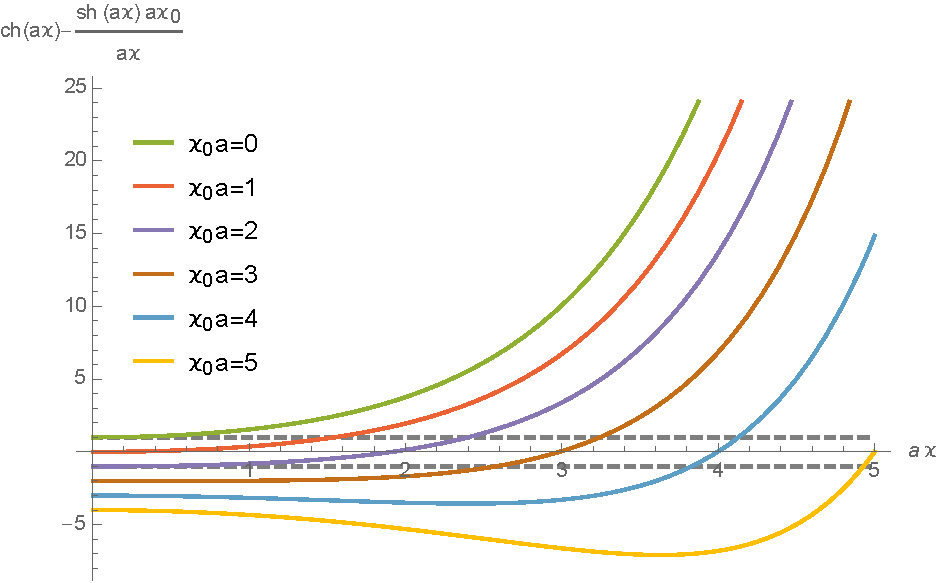
\includegraphics[width=0.8\textwidth]{7}
	\caption{Разрешённые зоны энергии (между штриховыми
	линиями) для различных $\kappa_0$} 
	\label{fig:7}
\end{figure}
В данном случае имеем лишь одну разрешённую зону для любых $\kappa_0$. При $\kappa_0 a\ll 1$ это будет зона  $\kappa a \approx 0$,
а при $\kappa_0 a \gg 1$ получаем
зону $\kappa_0 \approx \kappa$.
\end{sol}
\begin{problem}
	Рассмотреть вопрос о существовании связанного сферически симметричного состояния частицы в сферически симметричной потенциальной яме в пространстве одного, двух (качественно в импульсном представлении для мелкой ямы) и трёх измерений.
\end{problem}
\begin{sol}
	Рассмотрим сферически-симметричный локализованный потенциал $U(x)$ 
--- мелкую яму, которая может быть охарактеризована двумя масштабами:
глубиной $U_0$ и шириной $a$, удовлетворяющие соотношению
$U_0 \ll \hbar^2 /ma^2$. Далее будем обсуждать сразу случай
произвольной пространственной размерности $d=1,\,2,\,3.$ Также
положим $\hbar=1$.

Чтобы записать уравнение Шрёдингера в импульсном представлении,
необходимо его спроецировать на бра-вектор $\bra{\mathbf{p}}$, то есть
рассмотреть $\bra{\mathbf{p}}\widehat{\operatorname{H}}\ket{\psi}=
 E \braket{\mathbf{p}|\psi}$. Кинетическая энергия
 в таком случае запишется тривиально --- этот оператор
диагонален в импульсном представлении:
\[
	\bra{\mathbf{p}} \frac{\widehat{\operatorname{p}}^2}{
	2m}\ket{\psi}= \frac{\mathbf{p}^2}{2m}\psi(\mathbf{p})
.\] 
Потенциальная энергия не является диагональным оператором;
поэтому нам пригодятся её матричные элементы в этом базисе.
\begin{multline*}
	\bra{\mathbf{p}}U(\widehat{\operatorname{x}})\ket{\mathbf{p}'}= \bra{\mathbf{p}}U\left(\widehat{\operatorname{\mathbf{x}}}\right) \underbrace{\int d\mathbf{x} \ket{\mathbf{x}}\bra{\mathbf{x}}}_{\hat{\operatorname{\mathbb{I}}}}\ket{\mathbf{p}'}=
	\int d \mathbf{x} U(\mathbf{x}) \braket{\mathbf{p}|\mathbf{x}}\braket{\mathbf{x}|\mathbf{p}'}=\\=
	\int d\mathbf{x} U(\mathbf{x}) e^{-i (\mathbf{p}-\mathbf{p}')x}= U_{\mathbf{p}-\mathbf{p}'}
,\end{multline*} 
из чего мы заключаем, что эти матричные элементы тождественно
совпадают с преобразованием Фурье от потенциала. В таком
случае, потенциальная энергия записывается в импульсном
представлении в следующем виде:
\[
	\bra{\mathbf{p}}U(\widehat{\operatorname{\mathbf{x}}})
	\ket{\psi}= \bra{\mathbf{p}}U(\widehat{\operatorname{\mathbf{x}}}) \underbrace{\int (d \mathbf{p}') \ket{\mathbf{p}'}
	\bra{\mathbf{p}'}}_{\hat{\operatorname{\mathbb{I}}}}
	\ket{\psi}= \int (d \mathbf{p}') U_{\mathbf{p}-\mathbf{p}'}\psi(\mathbf{p}')
 ,\]
 где введено удобное обозначение $(d \mathbf{p})\equiv
 d^d \mathbf{p} /(2\pi)^d$. Таким образом, уравнение
Шрёдингера в импульсном представлении записывается в следующем
виде:
\[
	\frac{\mathbf{p}^2}{2m}\psi(\mathbf{p})+ \int
	(d\mathbf{p}')\psi(\mathbf{p}')U_{\mathbf{p}-\mathbf{p}'}
	= E \psi(\mathbf{p})
.\] 

Обсудим сперва некоторые общие свойства связанных состояний
в яме (предполагая, что они имеются). Для конкретности можно
говорить об основном состоянии.

Первое, что приходит в голову --- это то, что частица, находясь
в связанном состоянии, находится большей частью в яме
и масштаб пространственного изменения её волновой функции
равен её ширине $a$. В этом случае из соотношения
неопределённостей следует, что типичное значение её импульса
--- это $p \sim \hbar /a$, и типичное значение кинетической
энергии, связанной просто с пространственной локализацией
частицы в яме, равно $\left<\widehat{\operatorname{T}} \right>
 \sim \hbar^2 /ma^2$.

В случае мелкой ямы $U_0 \ll \hbar^2 /ma^2$. Откуда полная
энергия частицы $E = \left<\widehat{\operatorname{U}} \right>+
 \left<\widehat{\operatorname{T}} \right>\sim  -U_0 +\hbar^2 /ma^2>0$ и частица просто <<вылетит>> из ямы в состоянии непрерывного
спектра. Единственное разрешение полученного парадокса
--- это предположить, что типичный масштаб волновой функции
связанного состояния в мелкой яме $l\gg a$ (так, чтобы выполнялось
во всяком случае нестрогое неравенство $U_0\ge \hbar^2 /ml^2$).
Но это означает, что большая часть волновой функции частицы
располагается вне ямы. В таком случае, масштаб $l$ волновой
функции определяется уравнением Шрёдингера вне ямы, где
волновая функция экспоненциально затухает $\psi(x) \simeq e
 ^{-\kappa |x|}$, и $\kappa =l^{-1}$ непосредственно связан
с энергией связанного состояния $|E|= \hbar^2 \kappa^2 /2m$.
Полученное соотношение масштабов волновой функции и ямы в
действительности означает, что внутри ямы волновая функция
практически не меняется --- а значит, связанное состояние
(если оно имеется) нечувствительно к деталям потенциала.

Итак, масштаб волновой функции в координатно представлении
--- большой масштаб $\kappa^{-1}\gg a$ --- что из соотношения
неопределённостей означает, что в импульсном представлении,
напротив, волновая функция $\psi(p)$ является локализованной
вблизи нуля на малом масштабе $\sim \kappa$. С другой стороны,
масштаб $U(\mathbf{x})$ --- это $a \ll \kappa^{-1}$; в свою
очередь, масштаб $U_{\mathbf{p}-\mathbf{p}'}$ --- это большой
масштаб $a^{-1}$. Благодаря большой разнице в масштабах,
в свёртке $\int (d\mathbf{p}') \psi(\mathbf{p}')U_{\mathbf{p}-
\mathbf{p}'}$ основной вклад в интеграл приходит с $|\mathbf{p}'|
\le \kappa$, на котором функция $U_{\mathbf{p}-\mathbf{p}'}$ 
меняется слабо --- поэтому её можно вынести за интеграл
как <<медленную огибающую>>, положив в ней $\mathbf{p}'$ 
нулём. Это приводит нас к следующему приближённому уравнению:
\[
	\frac{p^2}{2m}\psi(\mathbf{p})+U_p \int
	(d\mathbf{p}')\psi(\mathbf{p}')=
	E \psi(\mathbf{p})\implies
	\psi(\mathbf{p})= -\frac{U_{\mathbf{p}}}{-E +\frac{p^2}{
	2m}}\int (d \mathbf{p}')\psi(\mathbf{p}')
\] 
(отметим, что поскольку мы имеем дело с ямой, то потенциал
$U(x)<0$; и поскольку мы имеем дело со связанным состоянием,
то $E= -|E|<0$). Данное уравнение --- алгебраическое, ведь
в правой части стоит интеграл от волновой функции,
который является константой. Последнее упрощение можно сделать,
заметив, что в произведении перед интегралом, опять-таки,
$U_\mathbf{p}$ является медленной огибающей, а  $(|E|+p^2 /2m)^{-1}$ --- относительно быстрозатухающей функцией, посему можно
вообще положить $p=0$. Наконец, проинтегрировав получившееся
уравнение по $(d\mathbf{p})$ и сократив на интеграл от волновой
функции, мы получаем следующее уравнение самосогласования
--- которое является уравнением на допустимые уровни
энергии:
\[
	|U_{\mathbf{p}=0}|\int \frac{(d\mathbf{p})}{|E|+
	\frac{\mathbf{p}^2}{2m}}=1
.\]
\begin{enumerate}
\item \emph{Случай одномерной ямы}.

При буквально нулевой энергии, этот интеграл расходится степенным
образом на малых импульсах, и сходится на больших ---
поэтому ожидается степенная зависимость от энергии. Подбирая
достаточно маленькую энергию, можно прийти к тому, что
знак равенства будет иметь место. В действительности же,
этот интеграл, разумеется, считается точно:
\[
	|U_{\mathbf{p}=0}|\sqrt{\frac{m}{2|E|}} =1\implies
	|E|= \frac{m}{2\hbar^2}\left| \int\limits_{-\infty}^{\infty} U(x)dx  \right| ^2
.\] 
\item \emph{Случай двумерной ямы}.

Интеграл расходится логарифмически на малых и на больших импульсах.
На больших импульсах очевидным образом интеграл нужно обрезать
на масштабах $~ 1 /a$, поскольку это уравнение было выведено
именно в таком предположении (это позволило нам заменить
$U_\mathbf{p}$ на $U_{\mathbf{p}=0}$; и поскольку интеграл
логарифмический, то он нечувствителен к этой обрезке
--- она меняет лишь константу под логарифмом), а на маленьких
--- масштабом  $\sqrt{2mE} $; сингулярность на малых энергиях
 оказывается слабой, логарифмической. Поэтому чтобы сделать
левую часть порядка единицы, уровень энергии требуется
сделать ну очень маленьким. Приступим теперь к непосредственному
вычислению:
\[
	\int \frac{d^2 \mathbf{p}}{(2\pi)^2} \frac{1}{
	|E|+ \frac{p^2}{2m}}= \int \frac{2\pi p\, dp}{4\pi^2}
	\frac{1}{|E|+ \frac{p^2}{2m}}\approx
	\frac{m}{\pi} \int\limits_{\sim \sqrt{mE} }^{~1 /a} 
	\frac{dp}{p}= \frac{m}{2\pi} \ln \frac{\#}{ma^2 |E|}
.\] 
Точность этого выражения следующая: число перд логарифмом
определено точно, а в силу неточности при  обрезании,
число под логарифмом ($\#$) неизвестно. Для его нахождения нужно
решать уравнение Шрёдингера точно; это число уже
определяется явным видом потенциала. Тем самым, решая уравнение
самосогласования, мы получаем (восстанавливая опять $\hbar $ 
по размерности):
\[
	|E|= \# \frac{\hbar^2}{m a^2} \exp \left( 
		-\frac{2\pi \hbar^2}{m}\left| \int U(\mathbf{r})d^2 \mathbf{r} \right|^{-1} 
\right) 
.\] 
Таким образом, мы определили уровень энергии в мелкой
двумерной яме с экспоненциальной точностью; и этот
уровень оказывается действительно экспоненциально мелким.
Ведущая асимптотика даётся этой самой экспонентой, которая
может быть оценена как $\exp \left( -\frac{\hbar^2 /ma^2}{U_0} \right) \lll 1$. Число же в предэкспоненте таким способом
определить нельзя.
\item \emph{Случай трёхмерной ямы}.

Исследуемый интеграл вообще не расходится на малых импульсах,
поэтому он практически не зависит от энергии.
На больших импульсах он может быть обрезан на масштабе $\sim 1 /a$; тем самым, весь интеграл оценивается как
\[
	\int \frac{(d\mathbf{p})}{|E|+ \frac{p^2}{2m}}\sim 
	m a^{-1}
.\] 
С другой стороны, $U_{p=0}\sim U_0 a^3$; тем самым вся комбинация
имеет порядок $\frac{U_0}{\hbar^2 /ma^2}\ll 1$. Из-за
слабой чувствительности интеграла к изменению энергии, сделать
это выражение порядка единицы изменяя энергию, невозможно и
уравнение самосогласования не имеет решений. Из чего мы заключаем,
что в трёхмерии в мелкой яме нет связанных состояний.
\end{enumerate}
%\begin{enumerate}
%	\item \emph{Случай одного измерения} был разобран в задаче \ref{prob:2}. Условию сферической симметричности в одномерном
%смысле будут удовлетворять только чётные решения. А они в
%свою очередь существуют в любой симметричной прямоугольной яме. 
%\item \emph{Случай трёх измерений}. Условие сферической симметрии
%состояния
%\[
%	\psi(x,\,y,\,z)=\psi(r)
%.\] 
%Лапласиан в сферических координатах
%\[
%	\Delta=\frac{1}{r^2} \partial_r (r^2 \partial_r)+
%	\Delta_{\phi,\,\theta}
%.\] 
%\begin{figure}[ht]
%    \centering
%    \incfig{8}
%    \caption{8}
%    \label{fig:8}
%\end{figure}
%Уравнение Шрёдингера
%\[
%-\frac{\hbar}{2m}\Delta \psi+U\psi=E\psi
%\]
%для участка I будет выглядеть как
% \[
%	 \frac{1}{r^2}\partial_r \left( r^2 \psi' \right) +
%	 \frac{2m}{\hbar^2}(E+U_0)=0 \implies
%	 \psi''+ \frac{2\psi'}{r}+ \frac{2m}{\hbar^2}(E+U_0)
%	 \psi=0
%.\] 
%Попробуем найти решение в виде $\psi(r)=r^\alpha g(r)$:
% \[
%	 \alpha(\alpha-1)r^{\alpha-2}g+2 \alpha r^{\alpha-1}
%	 g'+r^\alpha g''+2\alpha r^{\alpha-2}g+ 2r ^{\alpha-1}
%	 g'+ \frac{2m}{\hbar^2}(E+U_0)r^\alpha g=0
%.\] 
%\[
%	g''+\frac{g'}{r}(2\alpha+2)+g \left( \frac{\alpha(\alpha-1)+2\alpha}{r^2}+\frac{2m}{\hbar^2}(E+U_0) \right) =0
%.\] 
%При $\alpha=-1$ это уравнение значительно упрощается:
%\[
%	g''+\frac{2m}{\hbar^2}(E+U_0)g=0\implies
%	g(r)= A e^{ikr}+B e^{-ikr},\quad
%	k^2=\frac{2m}{\hbar^2}(E+U_0)
%.\] 
%Откуда
%\[
%	\psi_\text{I} (r)= A r^{-1}e^{ikr}+B r^{-1} e^{-ikr}
%.\] 
%Чтобы интеграл $\displaystyle \int \psi_\text{I}^* \psi_\text{I}
% dV$ сходился, необходимо,
%чтобы $A+B=0$. Откуда 
%\[
%	\psi_\text{I}(r)= C \frac{\sin kr}{r}
%.\] 
%Аналогично решаем стационарное уравнение Шрёдингера в 
%области II:
%\[
%	\kappa^2= \frac{-2mE}{\hbar^2};\quad
%	\psi_\text{II}(r)= \frac{D e^{-\kappa r}}{r}
%.\] 
%Условия сшивки при $r=r_0$
%\[
%\left\{
%\begin{aligned}
%	C \frac{\sin k r_0}{r_0}&= \frac{D e^{-\kappa r_0}}{r_0},\\
%	C\left(\frac{k \cos k r_0}{r_0}- \frac{\sin kr_0}{r_0^2}\right) &= D \left( \frac{-\kappa e^{-\kappa r_0}}{r_0}-
%	\frac{e^{-\kappa r_0}}{r_0^2}\right) .
%\end{aligned}
%\right.
%\] 
%\[
%	\frac{1}{r_0^2}\left( k \cos k r_0- \frac{\sin k r_0}{r_0} \right) = \frac{1}{r_0^2}\left( -\kappa \sin k r_0- \frac{\sin
%	k r_0}{r_0} \right) 
%.\] 
%\[
%k \cos k r_0= -\kappa \sin kr_0 \implies \tg kr_0= -\frac{kr_0}{
%\kappa r_0}
%.\] 
%\[
%\frac{1}{ \sin^2 kr_0}= \frac{\kappa^2}{k^2}+1=
%\frac{k_0^2}{k^2}\implies |\sin kr_0|=
%\frac{kr_0}{k_0  r_0} \text{ при } \tg kr_0<0
%.\] 
%Аналогично случаю одномерной ямы
%\end{enumerate}
\end{sol}
\begin{problem}
Найти уровни энергии трёхмерного изотропного гармонического
осциллятора и кратности их вырождения, разделяя переменные
в декартовых координатах. Обсудить связь задачи с моделью
ядерных оболочек и получить значения магических чисел 2, 8, 20.
\end{problem}
\begin{sol}
Потенциальная энергия трёхмерного изотропного гармонического
осциллятора даётся формулой
\[
	V(r)= \frac{1}{2}m \omega^2 r^2
 ,\]
где $\omega$ --- это угловая частота, равная $\sqrt{k /m} $.
Т.\:к. пространство состояний такой частицы --- это тензорное
произведение пространств состояний, связанных с отдельными
одномерными волновыми функциями, то стационарное уравнение
Шрёдингера для такой системы будет задаваться как
\[
	-\frac{\hbar^2}{2m} \left( \frac{\partial ^2 \psi}{\partial x^2} +\frac{\partial ^2\psi}{\partial y^2} +\frac{\partial ^2\psi}{\partial z^2}  \right) +\frac{1}{2}m \omega^2 (x^2+y^2+z^2)\psi=E\psi
.\] 
Разделяя переменные, получаем
\[
	E_{n_x,\,n_{y},\,n_z}= (n_x+n_y+n_z+ 3 /2) \hbar \omega
,\]
или $E_n=(n+3 /2)\hbar\omega$, где $n$ --- неотрицательное
целое число. Итак, энергетические уровни вырождены и кратность
вырождения равна числу различных наборов $n_x,\ n_y,\ n_z$,
удовлетворяющих условию
\[
n_x+n_y+n_z=n
 ,\] 
а именно
\[
	\sum_{n_x=0}^{n} (n-n_x+1)=\frac{(n+1)(n+2)}{2}
.\] 
Аналогично электронам, протоны внешней оболочки будут
относительно слабо притягиваться к ядру, если на данной
оболочке будет мало протонов, т.\:к. они находятся дальше
всех от ядра. Поэтому, ядра с полностью заполненной внешней
оболочкой будут иметь самую сильную энергию связи в сравнении
с другими ядрами с таким же полным числом протонов. Все
утверждения, сформулированные выше, также справедливы и для
нейтронов.

Это означает, что магические числа (по определению --- числа нуклонов, характеризующие
наиболее устойчивые ядра) следует ожидать в атомах с полностью
заполненной внешней оболочкой.

Из-за спина, кратность вырождения уровней энергии трёхмерного
гармонического осциллятора удваивается, после чего становится
равной $(n+1)(n+2)$. Откуда получаем выражение для нахождения
магических чисел
\[
	\sum_{n=0}^{k} (n+1)(n+2)= \frac{(k+1)(k+2)(k+3)}{3}
.\] 
Для $k=1$ получаем магическое число $2$, для 2 --- 8, для 3 ---
20.
%Кратность вырождения равна числу орбиталей на соответствующем
%энергетическом уровне. Так, число $s$-орбиталей равно $K(0)=1$,
%$p$-орбиталей --- $K(1)=3$, $d$-орбиталей --- $K(2)=6$.
%Также стоит отметить, что квантовое состояние электронов,
%отличающихся лишь направлением спина, также будет энергетически
%эквивалентно.
\end{sol}
\begin{problem}
Рассмотреть когерентные состояния одномерного гармонического
осциллятора. Вычислить распределение по числу квантов
в когерентном состоянии.
\end{problem}
\begin{sol}
Собственные векторы оператора уничтожения $\widehat{\operatorname{a}}\ket{z}=z\ket{z}$ образуют систему так называемых
когерентных состояний гармонического осциллятора, причём $z$ 
--- любое комплексное число. Вектор $\ket{z}$ можно представить
в виде разложения по системе собственных векторов гамильтониана
\[
\widehat{\operatorname{H}}= \frac{\widehat{\operatorname{p}}^2}{
2m} +\frac{m \omega^2 \widehat{\operatorname{x}}^2}{2}=
\hbar \omega\left( \widehat{\operatorname{a}}^+ \widehat{\operatorname{a}}+\frac{1}{2} \right) 
,\] 
где
 \[
	 \widehat{\operatorname{a}}= \frac{1}{\sqrt{2} } \left( 
	 \widehat{\operatorname{Q}}+i \widehat{\operatorname{P}}\right) ,\quad \widehat{\operatorname{a}}^+ =\frac{1}{\sqrt{2} }
	 \left( \widehat{\operatorname{Q}}-i \widehat{\operatorname{P}} \right) 
,\]
и $\widehat{\operatorname{Q}}=\widehat{\operatorname{x}} /x_0$,
$\widehat{\operatorname{P}}=\widehat{\operatorname{p}} /p_0$, т.\:е.
\[
	\ket{z}=\sum_{n}^{} C_n(z)\ket{n}
.\] 
И с учётом уравнения на собственные значения
\[
	C_n(z)= \braket{n|z}=\frac{1}{z}\braket{n|\widehat{\operatorname{a}}z}=\frac{1}{z}\braket{\widehat{\operatorname{a}}^+n|z}
,\] 
где мы воспользовались также определением эрмитово сопряжённого
оператора. По построению
\[
\widehat{\operatorname{a}}^+\ket{n}= \sqrt{n+1} \ket{n+1}
 ,\] 
так что получаем рекуррентное соотношение
\[
	z C_n(z)=\sqrt{n+1} C_{n+1}(z)
 ,\]
которое можно разрешить в явном виде
\[
	C_n(z)= \frac{z^n}{\sqrt{n!} }C_0(z)
.\] 
Разложение принимает вид
\[
	\ket{z}= C_0 (z) \sum_{n}^{} \frac{z^n}{\sqrt{n!} }\ket{n}=C_0(z) \sum_{n}^{} \frac{(z \widehat{\operatorname{a}}^+)^n}{n!}
	\ket{0}=C_0 (z) e^{z \widehat{\operatorname{a}}^+}\ket{0}
 ,\]
где мы использовали соотношение 
\[
	\ket{n}= \frac{(\widehat{\operatorname{a}}^+)^n}{
	\sqrt{n!} }\ket{0}
.\] 
Коэффициент $C_0(z)$ можно определить из условия единичной
нормировки состояния
\[
	\braket{z|z}=|C_0(z)|^2 \bra{0}e^{z^* \widehat{\operatorname{a}}}e^{z \widehat{\operatorname{a}}^+}\ket{0}=
		|C_0(z)|^2 \sum_{n}^{} \frac{(z^* z)^n}{n!}=1
 ,\]
где мы учли ортогональность стационарных состояний. Отсюда
\[
	|C_0(z)|^2 e^{|z|^2}=1\implies C_0(z)= e^{
	- \frac{|z|^2}{2}}
.\] 
Окончательно
\[
\ket{z}= e^{- \frac{|z|^2}{2}}e^{z \widehat{\operatorname{a}}^+}
\ket{0}= e^{-\frac{|z|^2}{2}}\sum_{n}^{} \frac{z^n}{\sqrt{n!} }
\ket{n}
.\] 
Очевидно, что в данном состоянии нет определённого значения
энергии. Вероятность обнаружить значении энергии $E_n$ 
\[
w_n=|\braket{n|z}|^2= e^{-|z|^2}\frac{|z|^n}{n!}
\]
определяется распределением Пуассона.
\end{sol}
\end{document}
